\documentclass[a4paper, 12pt]{report}
\usepackage[utf8]{inputenc}
\usepackage{microtype}
\usepackage{hyperref}
\hypersetup{
    colorlinks,
    citecolor=black,
    filecolor=black,
    linkcolor=black,
    urlcolor=black
}
\usepackage{glossaries}
\makeglossaries
\usepackage{enumitem}
\usepackage{rotating}
\usepackage[colorinlistoftodos]{todonotes}
\usepackage[most]{tcolorbox}
\usepackage{afterpage}
\usepackage{amsmath}
\usepackage{graphicx}
\usepackage{url}
\usepackage[Lenny]{fncychap}

 \renewcommand{\baselinestretch}{1.5}
 \usepackage{mathptmx}
 \usepackage{fancyhdr}
    \pagestyle{fancy}
    \fancyhf{}
    \chead{}
    \rfoot{\thepage}
    \lfoot{\tiny{Plateforme d'administration de boutique e-commerce avec intégration d'un outil BI. \\ Diana Birame Diabong}}
    \rhead{\fancyplain{}{\textit{\leftmark}}}
 \usepackage{tabularx}
 \usepackage{caption}
 \usepackage[frenchb]{babel}
 \usepackage{subcaption}
\addto{\captionsfrench}{
  \renewcommand{\mtctitle}{Sommaire}
  \renewcommand{\tablename}{Tableau}
  \renewcommand{\bibname}{Références}
}

\newcommand{\tabitem}{~~\llap{\textbullet}~~}
 \usepackage{graphicx}
 \usepackage{minitoc}
 \usepackage{float}
 \setcounter{secnumdepth}{3}
 \setcounter{tocdepth}{2}
  
 
 \title{Plateforme d'administration de boutique d'e-commerce avec intégration d'un outil BI.}
\author{Prénom Nom}
\date{}
\definecolor{myblue}{RGB}{51,51,153}
\newcommand\blankpage{%
    \null
    \thispagestyle{empty}%
    \addtocounter{page}{-1}%
    \newpage}
 
 
\newsavebox{\mybox}
\newlength{\mydepth}
\newlength{\myheight}
 
\newenvironment{sidebar}%
{\begin{lrbox}{\mybox}\begin{minipage}{\textwidth}}%
{\end{minipage}\end{lrbox}%
  \settodepth{\mydepth}{\usebox{\mybox}}%
  \settoheight{\myheight}{\usebox{\mybox}}%
  \addtolength{\myheight}{\mydepth}%
  \noindent\makebox[0pt]{\hspace{-40pt}\rule[-\mydepth]{1pt}{\myheight}}%
  \usebox{\mybox}}
 
 \newcommand{\HRule}{\rule{\linewidth}{0.4mm}} % Defines a new command for the horizontal lines, change thickness here  
 
 
\begin{document}

\begin{titlepage}

\centering % Center everything on the page
 
%----------------------------------------------------------------------------------------
%   HEADING SECTIONS
%----------------------------------------------------------------------------------------

\textsc{\normalsize \textbf{RÉPUBLIQUE DU SÉNÉGAL}}\\[0.15cm] % Name of your university/college

\includegraphics[scale=.1]{img/flag}\\[0.15cm]
\textsc{\small \textbf{UNIVERSITÉ CHEIKH ANTA DIOP DE DAKAR}}\\[0.15cm]

\includegraphics[scale=.2]{img/ucad}\\[0.15cm] % Include a department/university logo - this will require the graphicx package
\textsc{\small \textbf{ÉCOLE SUPÉRIEURE POLYTECHNIQUE}}\\[0.15cm] % Major heading such as course name
\textsc{\small {\textit {DÉPARTEMENT GÉNIE INFORMATIQUE}}}\\[0.15cm] % Minor heading such as course title

%----------------------------------------------------------------------------------------
%   TITLE SECTION
%----------------------------------------------------------------------------------------
\begin{tcolorbox}[colback=white,colframe=myblue]
\centering
 \textcolor{myblue}{\small{\textbf{MÉMOIRE DE FIN DE CYCLE}}}\\
\small{\textbf{Pour l’obtention du :} \\
\textbf{DIPLÔME D'INGÉNIEUR TECHNOLOGUE EN INFORMATIQUE}} % Title of your document
\end{tcolorbox}

\begin{tcolorbox}[colback=white,colframe=myblue]
\centering
\textbf{\small{SUJET}}: \\
\textcolor{red}{\textbf {Plateforme d'administration de boutique e-commerce avec intégration d'un outil BI.}} % Title of your document
\end{tcolorbox}

 
%----------------------------------------------------------------------------------------
%   AUTHOR SECTION
%----------------------------------------------------------------------------------------

\begin{tcolorbox}[colback=white,colframe=myblue]
\small{\textbf{\underline{Lieu de stage }}: \textcolor{myblue}{Terinnova} \quad \textbf{\underline{Période stage}}: \textcolor{myblue}{04/02/2019 - 30/06/2019}}\\
\centering \newline

\includegraphics[scale=.6]{img/terinnova.png} % Title of your document
\end{tcolorbox}

\begin{tcolorbox}[colback=white,colframe=myblue]
\begin{tabular}{lll}
Présenté et soutenu par & Encadrant & Maître de stage\\
Diana Birame DIABONG & Dr Mandicou BA & M. Alioune KANOUTÉ
\end{tabular}
\end{tcolorbox}


% If you don't want a supervisor, uncomment the two lines below and remove the section above
%\Large \emph{Author:}\\
%John \textsc{Smith}\\[3cm] % Your name

%----------------------------------------------------------------------------------------
%   DATE SECTION
%----------------------------------------------------------------------------------------
\begin{flushright}
{\small{\textcolor{myblue}{Année Universitaire : 2019-2021}}} % Date, change the \today to a set date if you want to be precise
\end{flushright}
\end{titlepage}
\thispagestyle{empty}
\clearpage\null

% Deuxieme page de garde

\begin{titlepage}

\centering % Center everything on the page
 
%----------------------------------------------------------------------------------------
%   HEADING SECTIONS
%----------------------------------------------------------------------------------------

\textsc{\normalsize \textbf{RÉPUBLIQUE DU SÉNÉGAL}}\\[0.15cm] % Name of your university/college

\includegraphics[scale=.1]{img/flag}\\[0.15cm]
\textsc{\small \textbf{UNIVERSITÉ CHEIKH ANTA DIOP DE DAKAR}}\\[0.15cm]

\includegraphics[scale=.2]{img/ucad}\\[0.15cm] % Include a department/university logo - this will require the graphicx package
\textsc{\small \textbf{ÉCOLE SUPÉRIEURE POLYTECHNIQUE}}\\[0.15cm] % Major heading such as course name
\textsc{\small {\textit {DÉPARTEMENT GÉNIE INFORMATIQUE}}}\\[0.15cm] % Minor heading such as course title

%----------------------------------------------------------------------------------------
%   TITLE SECTION
%----------------------------------------------------------------------------------------
\begin{tcolorbox}[colback=white,colframe=myblue]
\centering
 \textcolor{myblue}{\small{\textbf{MÉMOIRE DE FIN DE CYCLE}}}\\
\small{\textbf{Pour l’obtention du :} \\
\textbf{DIPLÔME D'INGÉNIEUR TECHNOLOGUE EN INFORMATIQUE}} % Title of your document
\end{tcolorbox}

\begin{tcolorbox}[colback=white,colframe=myblue]
\centering
\textbf{\small{SUJET}}: \\
\textcolor{red}{\textbf {Plateforme d'administration de boutique e-commerce avec intégration d'un outil BI.}} % Title of your document
\end{tcolorbox}

 
%----------------------------------------------------------------------------------------
%   AUTHOR SECTION
%----------------------------------------------------------------------------------------

\begin{tcolorbox}[colback=white,colframe=myblue]
\small{\textbf{\underline{Lieu de stage }}: \textcolor{myblue}{Terinnova} \quad \textbf{\underline{Période stage}}: \textcolor{myblue}{04/02/2019 - 30/06/2019}}\\
\centering \newline

\includegraphics[scale=.6]{img/terinnova.png} % Title of your document
\end{tcolorbox}

\begin{tcolorbox}[colback=white,colframe=myblue]
\begin{tabular}{lll}
Présenté et soutenu par & Encadrant & Maître de stage\\
Diana Birame DIABONG & Dr Mandicou BA & M. Alioune KANOUTÉ
\end{tabular}
\end{tcolorbox}


% If you don't want a supervisor, uncomment the two lines below and remove the section above
%\Large \emph{Author:}\\
%John \textsc{Smith}\\[3cm] % Your name

%----------------------------------------------------------------------------------------
%   DATE SECTION
%----------------------------------------------------------------------------------------
\begin{flushright}
{\small{\textcolor{myblue}{Année Universitaire : 2019-2021}}} % Date, change the \today to a set date if you want to be precise
\end{flushright}

\end{titlepage}
\newpage

\pagenumbering{roman}
\dominitoc
\chapter*{Dédicaces \markboth{Dédicaces}{}} 
\markboth{DÉDICACES}{}


\chapter*{Remerciements \markboth{Remerciements}{
Je rends grâce à ALLAH pour m’avoir accordé sa guidance. 
Paix et bénédictions sur Celui qu'Allah a rendu meilleur, Le mettant au-dessus de tous, sur sa Famille et ses Compagnons qui obtinrent les privilèges d’ALLAH 
J’adresse mes sincères remerciements à: 
M.Saalihou. M. NDIAYE, mon maître de stage pour son accueil chaleureux; Pr Ibrahima FALL mon encadreur pour sa disponibilité et ses conseils; Tout le corps professoral du département Génie Informatique; 
Toutes les personnes qui, de près ou de loin, ont contribué à la réalisation de ce document. 
}}
\markboth{REMERCIEMENTS}{}


\chapter*{Avant-propos \markboth{Avant-propos}{}} 


\tableofcontents
\chapter*{Sigles et Abréviations \markboth{Sigles et Abréviations}{}}

\listoffigures
\listoftables


\chapter*{Résumé \markboth{Résumé}{}}


\chapter*{Abstract \markboth{Abstract}{}}


\chapter*{Introduction \markboth{Introduction}{}} \mtcaddchapter 
« Derrière un petit clic pour un individu se cache un grand pas pour l’économie. » déclarait par Le New York Times suite à la première transaction à distance par carte bancaire effectuée par Phil Brandenberger en 1994 aux USA. Ce premier achat de 12,48 \$ pour un album de Sting représente la première pierre d'un édifice qui ne cesse de croître depuis. En effet l’émergence du commerce en ligne est directement liée à l’apparition du web au début des années 1990 qui n'a cessé de connaitre d’évolutions jusqu’à nos jours.


Avec l’arrivée de la pandémie de la covid-19, le commerce électronique a connu un véritable boom et donc il ne s’agit  non plus seulement pour les vendeurs d’être présent sur le web mais de passer à un niveau plus avancé c'est-à-dire d’anticiper pour mieux comprendre les besoins des utilisateurs et y répondre parfaitement dans le but de pouvoir supporter la concurrence en utilisant des approches comme la BI (Business Intelligence) ou informatique décisionnel en français.


Cette dernière permet de fournir aux e-commerçants des indicateurs et des analyses extrêmement précis qui leur permettent d'étudier en profondeur leur situation existante et de mieux anticiper pour l'avenir.


Terinnova, notre structure d’accueil a jugé nécessaire de proposer à son client Samson basé au USA une espace d’administration avec un outil BI intégré suite à la création de son site d'e-commerce qui lui permettra de gérer ses produits, traiter ses commandes, gérer ses utilisateurs, d’évaluer ses activités de vente et l’aider à la prise de décision. C’est dans ce sillage que nous allons essayer d’atteindre nos objectifs à travers ce travail qui nous a été confié qui s’intitule « Mise en place d’un système d’administration d’e-commerce et intégration d’un outil BI ».


Le document s’articule autour de trois grandes parties :
La première partie, intitulée « présentation générale », fait une description de notre structure
d’accueil Terinnova et la présentation générale de notre sujet .
La deuxième partie quant à elle renvoie à « la méthodologie et l’analyse ». Dans celle-ci,
nous expliquerons d’abord les différentes méthodologies d’analyse et de conception, ensuite
nous en choisirons une pour enfin procéder à l’analyse des besoins.
Enfin, la troisième et dernière partie intitulée « implémentation de la solution » décrit en
premier lieu la conception de la solution, en second lieu le choix des outils et technologies
adéquats, pour ensuite procéder à la réalisation de notre plate-forme et enfin nous présenterons
ce qui a été réalisé.
\pagenumbering{arabic}
\addcontentsline{toc}{chapter}{Introduction}


% CHAPITRE 1
\chapter{Présentation Générale}
\textit{\textbf{Resume:} }.
\setcounter{minitocdepth}{2}
\minitoc
\newpage
\section{Présentation de la structure d'accueil}
Dans cette partie nous allons dabord présenté la structure d'accueil et ensuite renseigné son domaine d'activité.
\subsection{Présentation de la Societe Terinnova}
  {En activité depuis 2020 Terinnova est une jeune entreprise sénégalaise ouverte à l’international, spécialisée dans la mise en œuvre de solutions informatiques répondant à toutes les problématiques liées à la gestion des systèmes d’informations et des systèmes d’infrastructures réseaux. Avec son équipe d’Ingénieurs professionnels, dynamiques et qualifiés, Terinnova accompagne les entreprises dans la réalisation de leurs objectifs visant à générer de la plus-value pour celles-ci. \\
  Terinnova a pour mission d’être à la pointe de l’utilisation, de la création, du développement et de la transformation des technologies avancées de l’information et de la communication, bâtir un réseau mondial de professionnels afin de créer pleine satisfaction et de la plus-value pour leurs clients à travers le monde et les aider à réussir par le truchement des services et solutions de qualité, en matière de technologies intelligentes et innovantes. 
  \\
  Cette startup est portée dans toutes leurs actions par leurs valeurs, socles du respect de l'engagement vis à vis de l’humanité, vis à vis de leurs clients, vis à vis de leurs partenaires, vis à vis du continent africain.}
\subsection{Domaines d'activités}
{ Les services que Terinnova proposent sont assez larges. On peut en citer quelques : 


\textbf{--- Digital Consulting : }
\\
Terinnova proposent un service de conseil qui accompagne les entreprises dans leurs transformation digitale, leur aide à se maintenir dans un marché mondial en constante évolution et en phase avec les dernières tendances technologiques. Du E-Commerce à la gestion des produits et des données en passant par le CRM, nous mettons en œuvre des solutions numériques centrées sur l'utilisateur, dont le succès à long terme est assuré par des experts en conception et développement. Grâce à ces compétences techniques et de processus étendues, vos idées novatrices se transformeront rapidement en résultats effectifs et tangibles.

\textbf{--- Software Engineering :} 
\\
Transformer des idées en résultats commerciaux tangibles nécessite un solide bagage technique et une expertise dans tous les secteurs. Grâce à de solides pratiques de gestion et à une expertise en ingénierie des logiciels, TERINNOVA peut vous guider en toute sécurité dans la transformation numérique, en gardant votre entreprise agile, de l'élaboration des exigences détaillées au déploiement et à l'optimisation. Quelle que soit la complexité de votre vision, nous lui donnerons vie grâce à des solutions d'ingénierie numérique de qualité. 

\textbf{--- Big Data \& Business Aanalytics:}  
\\
L’analyse commerciale « Business Analytics» se concentre sur un point essentiel, à savoir l'analyse financière et opérationnelle de l'entreprise. D'un autre côté, l'analyse « Big Data » aide à analyser une plus large gamme de données provenant de toutes les sources d'informations possibles et aide l'entreprise à prendre de meilleures décisions. 

\textbf{--- Infrastructure :}
\\
Dans ce monde numérique et de cloud, les performances de votre entreprise sont étroitement liées au bon fonctionnement de votre infrastructure informatique. Une infrastructure agile et intelligente vous aide non seulement à vous adapter rapidement au changement, elle stimule également l'innovation et permet d'acquérir de nouveaux modèles commerciaux. 
}
\section{Présentation du sujet}
{Dans cette section nous présentons de manière explicite le sujet de notre mémoire «\textbf{mise en place d’un système d’administration d’e-commerce avec intégration d’un outil BI}». Nous allons parler du contexte dans lequel s’inscrit notre sujet, de la problématique et des objectifs à atteindre.}
\subsection{Contexte}
{Au cours de ces dernières années, l'e-commerce a totalement révolutionné le secteur de l’économie numérique et s’est fortement intégré dans les habitudes des consommateurs. Cette révolution a été accélérer par l’arrivée du covid-19. Alors que le confinement devenait la nouvelle normalité, les entreprises et les consommateurs se tournaient de plus en plus vers le numérique, vendant et achetant davantage de biens et de services en ligne. 

En e-commerce, il existe de nombreux indicateurs pour aider les marchands à piloter leur activité et à optimiser leur gestion. Des chiffres qui leur permettent à la fois de dresser un état des lieux en temps réel mais également de mesurer l’efficacité des actions passées, d’analyser les résultats et de préparer les stratégies à venir. En effet, pour obtenir une vision plus fine et plus complète, il est nécessaire d’aller plus loin et d’accéder à des données et à des analyses plus poussées, à travers notamment la Business Intelligence. Ainsi, avec cette dernière, les marchands disposent d’une valeur ajoutée sans précédent pour mieux vendre et augmenter leurs revenus ! Elle leur permet de mieux connaître leur activité et leurs clients et d’optimiser leur fonctionnement à tous les niveaux.

C’est dans ce contexte que s'inscrit notre sujet, un projet important pour Terinnova qui est la création d'une application web d’e-commerce pour son client Samson basé aux USA, une marque de vêtements. Grâce à cette application Samson pourra gérer ses produits, traiter ses commandes, gérer ses clients, évaluer ses activités de vente et prendre éventuellement des décisions.}
\subsection{Problématique}
{La plupart des plateformes d’e-commerce sont conçu avec des systèmes de gestion de contenu comme wordpress, wix... qui ont souvent des espaces d’administration chargée de fonctionnalités souvent inutiles pour le e-commerçant. En effet cela a un impact sur l’utilisation des fonctionnalités indispensables comme la gestion des stocks, le traitement des commandes...etc.

De plus on ne pourra pas exploiter les données provenant des activités de vente car on n'a pas le contrôle dessus et donc on ne pourra pas établir de stratégie pour mieux vendre et augmenter ses revenus.}
\subsection{Objectifs}
{Notre objectif principal est de permettre à Samson d’avoir une application web sur mesure pour la gestion de son e-commerce. En effet cet outil permettra de faciliter l’exploitation des données de l’application et d’avoir un aperçu sur ses revenus annuels. Plus spécifiquement il s’agit d’avoir un outil pour s’assurer :
\begin{itemize}
  \item de la gestion des produits 
  \item de la gestion des commandes
  \item de la gestion des clients
  \item et de l'analyse de donnée
\end{itemize} 
}

\section{ Méthodologie de travail}
\textit{\textbf{Résumé:} }
\setcounter{minitocdepth}{1}
\minitoc

\subsection{Méthodologie de développement}
Une méthodologie de développement représente un élément indispensable pour mieux organiser le projet et espérer aboutir aux résultats attendus. Ainsi, nous allons présenter le choix de la méthode de développement le plus convenable qu’on a emprunté pour la réalisation de notre projet. 
\subsubsection{Pourquoi une méthodologie de développement de logiciel ?}
Une méthode de travail pour un logiciel est une manière de structurer, planifier et contrôler le processus de développement. 
\\
Pour mieux comprendre ce qu'est une méthodologie de développement, voici quelques termes qui sont souvent utilisés dans ce domaine : \\
-- \textbf{Méthodologie :} une collection de principes et/ou pratiques,\\ 
-- \textbf{Famille de méthodologies :} un ensemble de méthodes alternatives qui coexistent,\\
-- \textbf{Framework :} un squelette qui a besoin d'être développé et personnalisé avant utilisation,\\ 
-- \textbf{Modèle :} une description qui doit être implémentée par une méthode, famille, ou Framework.\\
Des études comme celles menées par le Standish Group (un groupe dont la mission est la recherche ciblant l’amélioration de performance des projets logiciels) ont démontré qu’il y a 25 ans : 

\begin{itemize}
  \item \textbf{16,2\%} de tous les projets MIS étaient terminés dans les délais et dans les limites du budget, selon ce que le groupe Standish a appelé à juste titre le rapport CHAOS.  
  \item \textbf{52,7\%} étaient en retard et dépassaient le budget. ,
  \item \textbf{31,1\%} ont été carrément annulés. Les deux principales raisons étaient alors le manque de participation des utilisateurs et des exigences incomplètes. 
\end{itemize} 

En 2017 il y a eu amélioration du taux de réussite, qui est passé de 16,2\% à 29\%. Certains projets ont même atteint 62\%.  

\begin{figure}[!h]
\centering
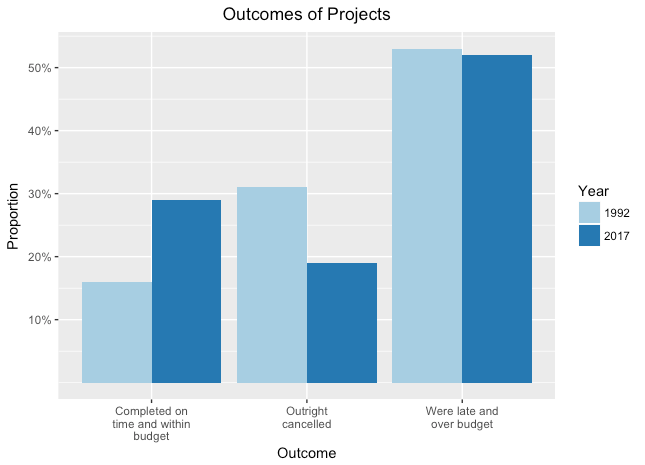
\includegraphics[width = 1\linewidth]{img/outcome-of-projects.png}
\caption{Résultats des projets}
\end{figure}

\textbf{Qu’est-ce qui a changé en 25 ans ?} \\
Un rapport Wrike de 2015 s'est penché sur l'utilisation d'une méthodologie et a trouvé que celles qui ont eu plus de succès, 38\% contre 31\%.  Ceux qui ont utilisé une méthodologie étaient toujours en retard de 72\%, 29\% n'ont pas respecté la portée, 32\% n'ont pas respecté les exigences de qualité, 40\% n'ont pas respecté les bénéfices attendus et les chiffres sont encore pires pour les projets qui n'ont pas utilisé de méthodologie.\\
Nous allons présenter certaines des plus importantes méthodologies concernant le développement de logiciel dans les lignes qui suivent. 

\subsubsection{Les méthodes classiques}
\begin{itemize}
  \item \textbf{Modèle en cascade :} Le modèle en cascade est un processus d'implémentation séquentielle, souvent utilisé dans le processus de développement de logiciel. 
\begin{figure}[!h]
\centering
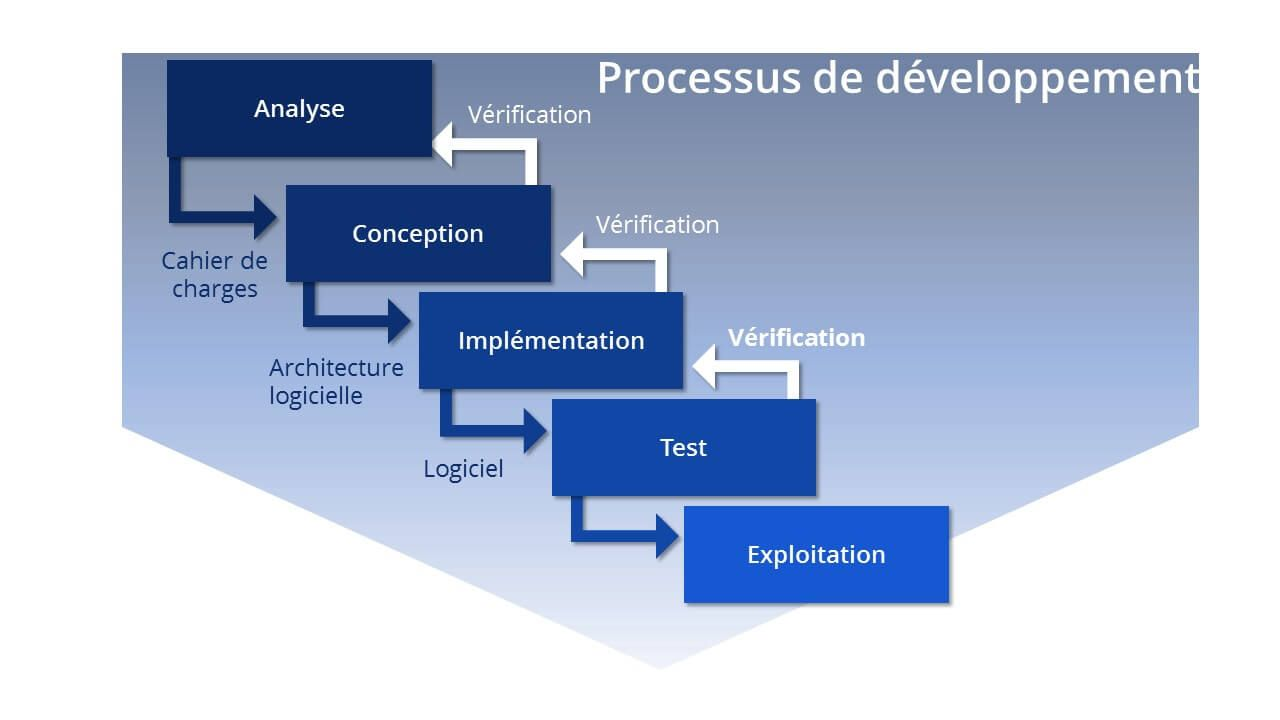
\includegraphics[width = 1\linewidth]{img/wasserfallmodell.jpg}
\caption{Différentes phases du modèle en cascade}
\end{figure}
En pratique, plusieurs versions du modèle en cascade sont utilisées. Les modèles les plus courants divisent les processus de développement en cinq phases. Les phases 1, 2 et 3 sont parfois regroupées en une seule et même phase, qualifiée d’analyse des besoins. \\
\textbf{ Analyse :} toutes les exigences possibles du système prévu sont établies. \\
\textbf{ Conception :} les exigences de la première étape sont étudiées et la conception du projet est élaborée. \\
\textbf{ Implémentation :} après que la conception est faite, le travail est divisé en modules et la vraie implémentation du code commence. Le système est premièrement développé en petits programmes, appelés "unités" qui vont alors être intégrés dans la phase suivante. Chaque unité est développée et testée afin d'assurer qu'elle rencontre les spécifications. \\
\textbf{ Test :} les unités développées dans la phase précédente sont intégrées et testées, et le système, vu comme un ensemble, se comporte en accord avec les spécifications. Après que le test soit réussi, le produit est livré au bénéficiaire.\\
\textbf{ Exploitation (livraison, maintenance, amélioration) :} en général, les problèmes concernant les logiciels se produisent après que le produit final commence à être utilisé, de cette manière les problèmes seront résolus après le lancement du produit. \\

\begin{table}[H]
\begin{tabular}{|p{6cm}|p{6cm}|} 
\hline  
\centering \textbf{Avantages} & \raggedright  \textbf{Inconvénients} \tabularnewline  
\hline
\raggedright Une structure simple grâce à des phases de projet clairement délimitées.&  Les projets complexes ou à plusieurs niveaux ne peuvent que rarement être divisés en phases de projet clairement définies.   \tabularnewline  
\hline  
\raggedright Une bonne documentation du processus de développement par des étapes clairement définies. & Une faible marge pour les ajustements du déroulement du projet en raison d’exigences modifiées. \tabularnewline
\hline
\raggedright Les coûts et la charge de travail peuvent être estimés dès le début du projet. & L’utilisateur final est uniquement intégré dans le processus de production après la programmation. \tabularnewline
\hline
\raggedright Les projets structurés d’après le modèle en cascade peuvent être représentés facilement sur un axe temporel. & Les erreurs sont parfois détectées uniquement à la fin du processus de développement. \tabularnewline
\hline
\end{tabular}
\caption{Avantages et inconvénients du modèle en cascade}
\end{table}

  \item \textbf{Cycle en V :} \\
  Le cycle en V est une méthode traditionnelle de gestion de projet conçue tout d’abord pour l’industrie puis adaptée à l’informatique en 1980. C’est une évolution du cycle en cascade qui manquait de réactivité. Il évite les retours en cas d’anomalie rencontrées. Il est composé d’une phase descendante puis montante, la phase montante envoie des informations vis-à-vis de la phase descendante. \\
  \begin{figure}[!h]
    \centering
    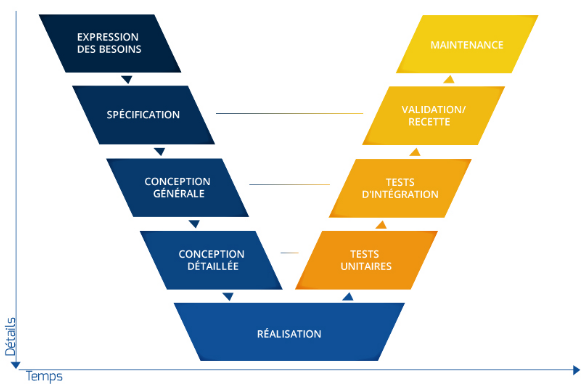
\includegraphics[width = 1\linewidth]{img/cycle-en-V.png}
    \caption{Cycle en V}
 \end{figure}\\
  Le cycle en V est un cycle composé de 3 grandes phases contenant 8 étapes de conception d’un produit : \\
  \textbf{La phase de conception :} analyse des besoins et faisabilité, spécifications, conception Architecturale, conception détaillée 

   \textbf{La phase de réalisation :} codage, tests unitaires 

   \textbf{La phase de validation :} tests d’intégration, test de validation, recette. 
  
\begin{table}[H]
\begin{tabular}{|p{6cm}|p{6cm}|} 
\hline  
\centering \textbf{Avantages} & \raggedright  \textbf{Inconvénients} \tabularnewline  
\hline
\raggedright La mise en œuvre du projet est sécurisée dans la mesure où chaque phase ne commence qu'à partir du moment où la précédente est terminée. &  La méthode du cycle en V n’est pas adaptée pour le changement.   \tabularnewline  
\hline  
\raggedright Elle permet de bien préparer en amont les phases de spécification.  & Le cycle en V ne prévoit pas de nouvelles décisions lors d’un cycle. Les changements doivent se faire entre deux cycles en V.  \tabularnewline
\hline
\raggedright En face de chaque phase de spécification, est mis en place un système de vérification, ce qui assure un meilleur produit au final.  &  \tabularnewline
\hline
\end{tabular}
\caption{ Avantages et inconvénients du cycle en V}
\end{table}

 \item  \textbf{Modèle de prototype :}\\
Le but de ce prototype est de contrer les deux premières limitations du modèle en cascade. Au lieu de définir les exigences avant de pouvoir concevoir et déployer, un prototype est lancé pour comprendre les exigences. Il est développé sur la base des exigences actuellement connues. Le développement de prototype implique les phases de conception, d'implémentation et test, mais celles-ci ne sont pas très rigoureuses ou formelles. \\
\begin{figure}[H]
\centering
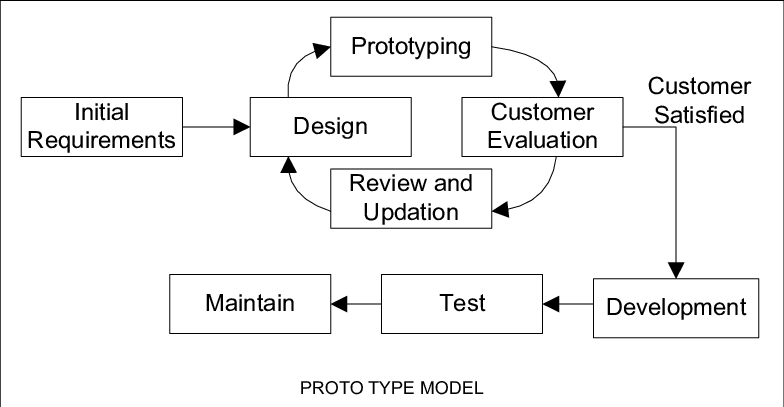
\includegraphics[width = 1\linewidth]{img/prototype-model.png}
\caption{Différentes phases du modèle de prototype }
\end{figure}
A travers le prototype, le client comprend mieux comment le produit fonctionne, puisqu'il interagit avec lui tout au long du cycle développement. \\
Ce modèle est préféré entre beaucoup de systèmes larges et compliqués, pour lesquels il est difficile de comprendre les exigences depuis le début. Dans ce type de situations, l’accès du client au prototype fournit une contribution significative pour comprendre et définir les caractéristiques.
\begin{table}[H]
\begin{tabular}{|p{6cm}|p{6cm}|} 
\hline  
\centering \textbf{Avantages} & \raggedright  \textbf{Inconvénients} \tabularnewline  
\hline
\raggedright Les utilisateurs sont directement impliqués dans le développement.  &  Ce modèle peut augmenter la complexité du système, ou peut s'étendre au-delà des limites fixées.    \tabularnewline  
\hline  
\raggedright Il encourage les utilisateurs à changer leurs exigences tout au long du cycle d'implémentation. & Analyse insuffisante du projet dans son entièreté.   \tabularnewline
\hline
\raggedright Vu qu'un modèle fonctionnel du système est mis à disposition, les utilisateurs peuvent mieux comprendre comment il fonctionne.   & Les développeurs peuvent devenir attachés à un prototype dont le développement a investi beaucoup de temps et va tendre à transformer le prototype en produit final même si l'architecture de base n'est pas la bonne.  \tabularnewline
\hline
\raggedright Les erreurs peuvent être détectées plus tôt. & Implémenter un prototype prend beaucoup de temps. \tabularnewline
\hline
\raggedright Le retour d'information est plus rapide, ce qui amène à de meilleures solutions. & \tabularnewline
\hline
\raggedright Temps et coûts réduits & \tabularnewline
\hline
\end{tabular}
\caption{Avantages et inconvénients du modèle de prototype}
\end{table}

\item \textbf{Modèle en spirale :}
Les étapes d'itération pour le modèle en spirale sont les suivantes : \\
\textbf{Les exigences :} du système sont définies de la manière la plus détaillée possible. Cela implique d'habitude d'interroger un nombre d'utilisateurs représentant les utilisateurs internes et externes du système aussi bien que d'autres problèmes ;\\ 
\textbf{Une conception :} préliminaire pour le système est créée. Cette phase est la plus importante du modèle. À cette étape, toutes alternatives possibles (et disponibles), qui peuvent aider à développer un projet coûteux, sont analysées et les stratégies d'approches sont décidées ; \\
\textbf{Un premier prototype :} du nouveau système dans la conception préliminaire est développé. C'est d'habitude un système à échelle réduite et est une approximation des caractéristiques du produit final ;\\ 
\textbf{Un second prototype est développé}, comme suit :\\
    -- Evaluer le premier prototype en termes de forces, faiblesses et risques,\\
    -- Définir les exigences pour le second prototype, \\
    -- Planifier et conceptualiser le second prototype, \\
    -- Développer et tester le second prototype. \\
\end{itemize} 
\begin{figure}[H]
    \centering
    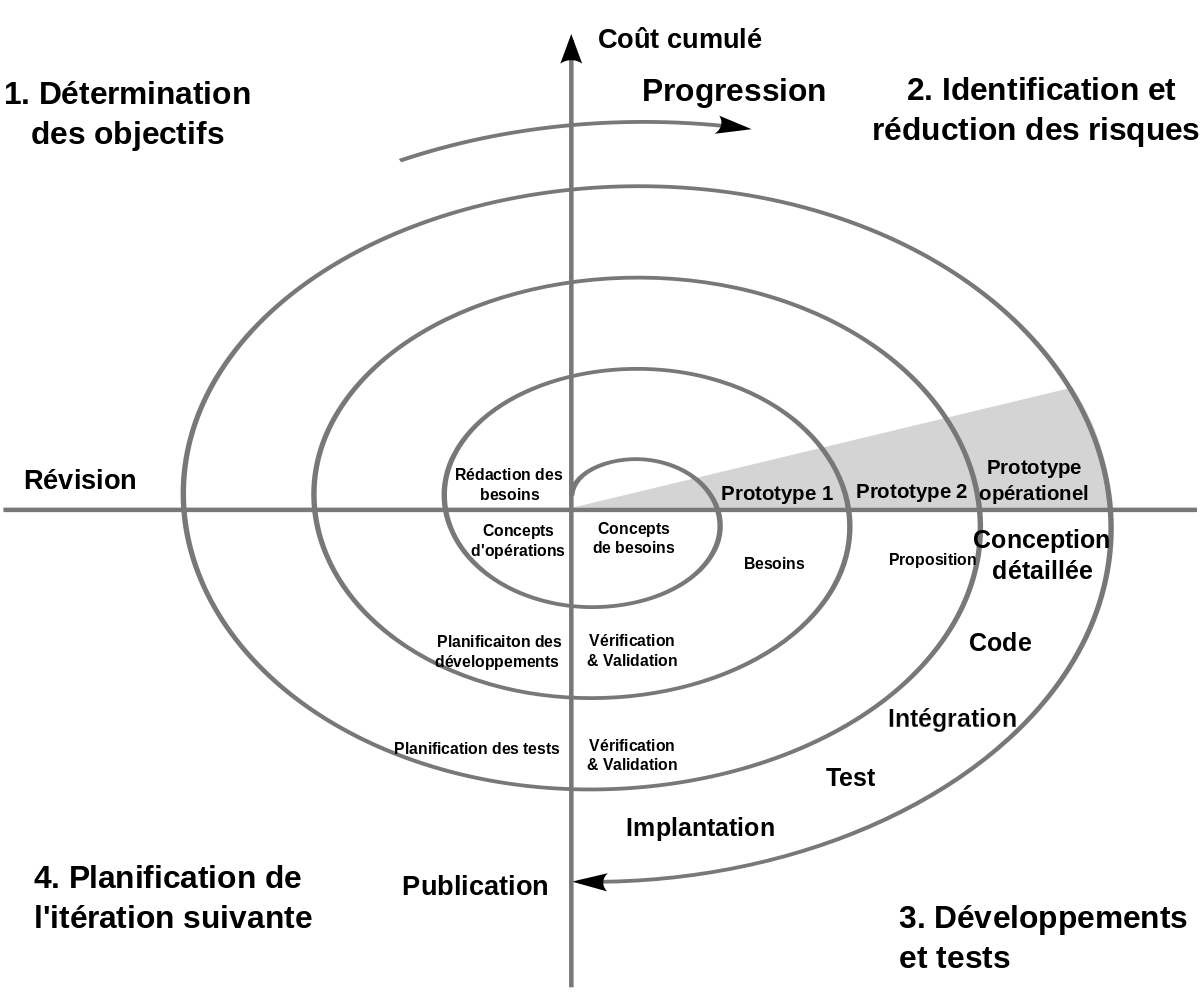
\includegraphics[width = 1\linewidth]{img/model-spirale.png}
    \caption{Étapes d’itération du modèle en spirale}
\end{figure}
\begin{table}[H]
\begin{tabular}{|p{6cm}|p{6cm}|} 
\hline  
\centering \textbf{Avantages} & \raggedright  \textbf{Inconvénients} \tabularnewline  
\hline
\raggedright Démontre une attitude proactive envers les risques, avec une supposition explicite des risques et leur résolution.  &  Presque impossible d'estimer le temps et les coûts depuis le début.   \tabularnewline  
\hline  
\raggedright Très flexible  &  \tabularnewline
\hline
\end{tabular}
\caption{Avantages et inconvénients du modèle en spirale}
\end{table}

\subsubsection{Les méthodes agiles }
La méthodologie Agile s'oppose généralement à la méthodologie traditionnelle Waterfall. Elle se veut plus souple et adaptée, et place les besoins du client au centre des priorités du projet. 

A l'origine, cette approche a été créée pour les projets de développement web et informatique. Aujourd'hui, la méthode Agile est de plus en plus répandue car elle est adaptable à de nombreux types de projets, tous secteurs confondus. 

La méthodologie Agile est basée sur un développement itératif et incrémenté ou les caractéristiques et solutions viennent de la collaboration entre équipes organisées individuellement, mais avec le même but commun. 

Suite à l'observation d'un taux d’échec élevé des projets dans les années 1990, 17 experts en développement logiciel se réunissent aux Etats-Unis en 2001 afin de mettre en commun leurs méthodes respectives. Le « Manifeste Agile » (Agile Manifesto en anglais) naît de cette rencontre et détermine les valeurs et les principes fondamentaux de la méthode Agile. 

Une plus grande implication du client et une meilleure réactivité des équipes face à ses demandes sont au cœur de la méthode Agile. Ce manifeste prône les 4 valeurs fondamentales de la méthodologie: \\
\textbf{-- L'équipe}, soit des individus et des interactions plutôt que des processus et des outils ; \\
\textbf{-- L’application}, c'est-à-dire des fonctionnalités opérationnelles plutôt que de la documentation exhaustive ; \\
\textbf{-- La collaboration} avec le client plutôt que la contractualisation des relations ; \\
\textbf{-- L’acceptation} du changement plutôt que le suivi d'un plan. \\

De ces valeurs découlent les 12 principes généraux suivants : \\
-- Satisfaire les clients en délivrant continuellement et rapidement un logiciel ; \\
-- Accueillir les changements d'exigences, même tard dans l'implémentation ;\\ 
-- Un logiciel utilisable est délivré fréquemment (quelques semaines) ; \\
-- Un logiciel utilisable est la principale mesure de progrès ; \\
-- Développement durable, capable de garder un rythme stable; \\
-- Coopération rapprochée entre développeurs et clients ; \\
-- Conversation en face à face est la meilleure façon de communiquer ; \\ 
-- Les projets sont construits par des personnes motivées et crédibles ; \\
-- Simplicité ; \\
-- Équipes organisées individuellement ; \\ 
-- Adaptation aux circonstances changeantes ; \\ 
-- Attention constante à l'excellence technique et bonne conception. \\
\begin{figure}[H]
    \centering
    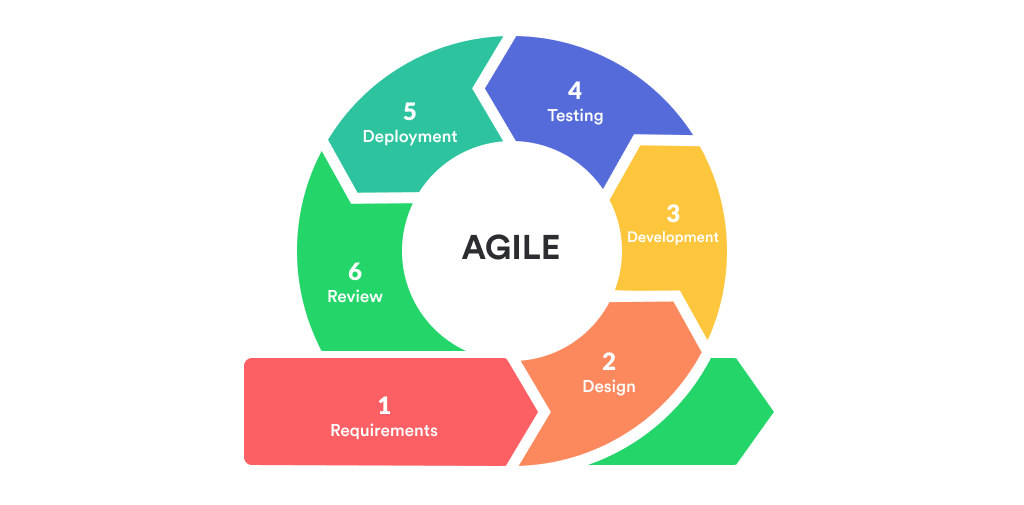
\includegraphics[width = 1.2\linewidth]{img/agile.jpg}
    \caption{Méthodologie Agile}
\end{figure}
SCRUM et eXtrem Programming (XP) sont parmi les méthodes agiles les plus importantes. 
\begin{itemize}
    \item \textbf{eXtrem programming :}\\
    Extreme Programming, ou XP, est une méthode agile de gestion de projet particulièrement bien adaptée aux projets de développement informatique. Elle a été conçue par Kent Beck pour accélérer les développements alors qu’il travaillait pour la société Chrysler. L’idée lui est venue alors qu’il devait intervenir sur un logiciel de paie écrit en langage Smalltalk ayant accumulé une dette technique considérable, le rendant particulièrement complexe à maintenir et à faire évoluer. 

Le principe fondamental de la méthode XP est de faire collaborer étroitement tous les acteurs du projet et d’opter pour des itérations de développement très courtes. La planification des tâches reste très souple et l’estimation des charges simplifiée par des projections à très court terme. Ainsi la correspondance entre ce qu’attend le client et les réalisations est garantie. Les fonctionnalités sont livrées régulièrement, afin d’être testées et validées au travers de prototypes opérationnels. 
L’eXtreme Programming préconise également le travail en binôme des développeurs, facilitant ainsi la production d’un code simple, facilement lisible et maintenable. 


Un certain nombre de règles doit s’appliquer systématiquement aux développements réalisés dans le cadre de la méthode agile XP : \\
-- La relecture du code doit être faite systématiquement. \\
-- Les tests doivent être systématiques, complets, et réalisés à la fin de chaque étape. \\
-- L’amélioration du code est faite tout au long de l’avancement des itérations. \\
-- Les modifications sont publiées souvent de façon à permettre à tous d’avancer rapidement. \\
-- La solution la plus simple est toujours privilégiée. \\
-- Les termes utilisés doivent être parfaitement définis de façon à ce que la compréhension du projet soit la même pour tous les intervenants. \\

L’application de ces règles va permettre au fur et à mesure de  l’avancement du projet de mettre en place des bonnes pratiques de  développement, de permettre un apprentissage et une montée en  compétences rapides, et au final de mettre en place un processus d’amélioration continue. 

\begin{figure}[H]
    \centering
    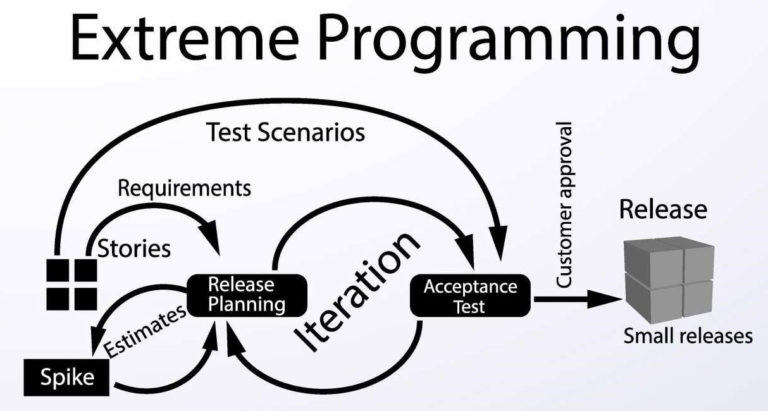
\includegraphics[width = 1\linewidth]{img/xp.jpg}
    \caption{Méthodologie eXtrem Programming}
\end{figure}

Extreme Programming, ou XP, décrit 4 activités basique qui sont effectuées pendant le processus de développement du logiciel : \\
\textbf{-- Écriture du code} - Les partisans d'XP pensent que la seule production vraiment importante du processus de développement est le code. Sans le code, il n'y a pas de produit viable. \\
\textbf{-- Testing} - Dans l'approche XP si un petit test peut éliminer quelques erreurs, plus de test peuvent éliminer plus d'erreurs. \\
\textbf{-- Écoute} - Les développeurs doivent écouter ce que les clients veulent du système. Vous devez comprendre ces exigences assez pour donner un retour au client sur les problèmes techniques qui peuvent être résolus (ou pas). \\
\textbf{-- Conception} - Promeut la création d'une structure logique pour le projet, pour éviter un large nombre de dépendances dans le projet et faciliter la mise en place de n'importe quel changement. 

\begin{table}[H]
\begin{tabular}{|p{6cm}|p{6cm}|} 
\hline  
\centering \textbf{Avantages} & \raggedright  \textbf{Inconvénients} \tabularnewline  
\hline
\raggedright XP livre une conception et logiciel de qualité pendant un développement réaliste.  & Extreme Programming est dur à accomplir - il est difficile d'obtenir un nombre de développeur qui accepteront cette pratique et cela prend beaucoup de discipline pour tout le monde pour compléter un projet avec cette approche.  \tabularnewline  
\hline  
\raggedright Un haut niveau de qualité du fait du test de tous les aspects.  &  Le logiciel d'aujourd'hui est très large et complexe, ce qui rend difficile de concevoir incrémentalement avec XP  \tabularnewline
\hline
\raggedright Le travail d'équipe est encouragé - Les développeurs travaillent par pair ou les deux ont un seul écran et un seul clavier.  &  XP se focalise sur le remaniement pendant le processus de mise en place, ce qui peut réduire la productivité des problèmes   \tabularnewline
\hline
\raggedright La satisfaction du client est augmenté dû à la manière dont ses exigences sont comprises.  & Développement basé sur le code, au lieu d'être basé sur la conception. \tabularnewline
\hline
\raggedright La conception est simple - La conception n'est pas faite pour quelque chose dans le futur mais, pour le présent. & Manque de documentation sur la conception . \tabularnewline
\hline
\raggedright Cas de test facile à comprendre. &  \tabularnewline
\hline
\end{tabular}
\caption{Avantages et inconvénients méthode XP }
\end{table}

\item \textbf{Scrum}\\
La méthode agile Scrum particulièrement destinée à la gestion de projets informatiques tient son nom du monde du rugby. Le principe de Scrum est de pouvoir modifier la direction prise par le projet au fur et à mesure de son avancement. 

La méthodologie demande à ses acteurs d'être soudés dans l'accomplissement d'un projet, dans l'atteinte d'un but. Elle utilise une procédure dite itérative (une itération est appelée sprint). Chaque partie fonctionnelle du produit découle d’une itération ou sprint. C’est une méthodologie qui est principalement basée sur la gestion des ressources humaines et peut être adaptée à d’autres contextes où il existe un besoin de travailler en équipe. Scrum peut donc être vu comme le cadre de développement venant par exemple appuyer des pratiques XP. Scrum suppose donc une intense collaboration entre les différentes personnes impliquées. 
\begin{figure}[H]
    \centering
    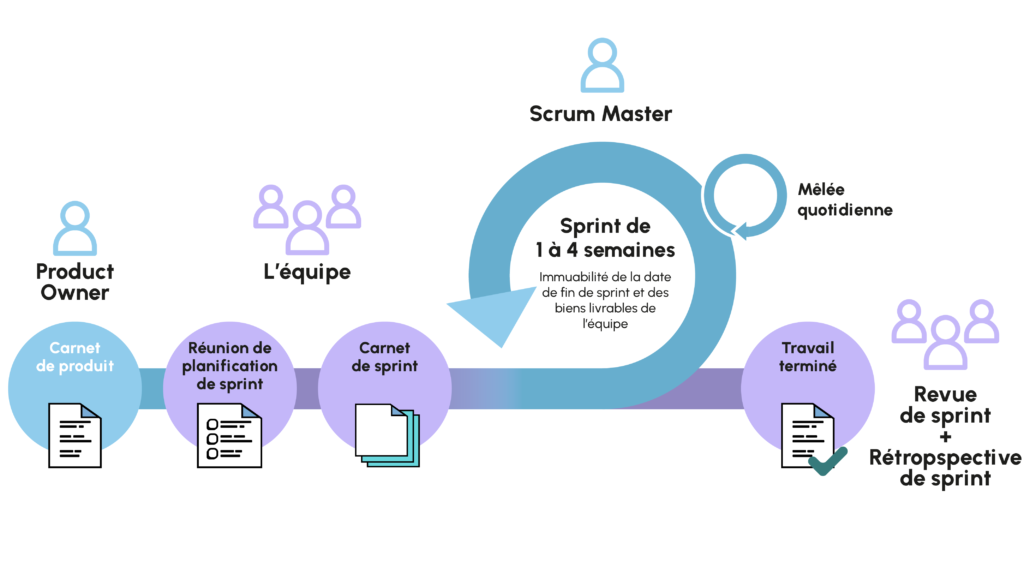
\includegraphics[width = 1\linewidth]{img/srum.png}
    \caption{Méthodologie SCRUM}
\end{figure}

Le processus Scrum repose sur deux journaux ou « backlog»: 

\textbf{- Product Backlog :} liste regroupant les exigences du client. Il évolue au cours du développement pour prendre  en charge au mieux les besoins du client. 

\textbf{- Sprint Backlog :} recense les tâches du Sprint en cours. 

Durant chaque "sprint" (habituellement 2-4 semaines), l'équipe (team) crée un livrable. L'ensemble des fonctionnalités du sprint viennent du "backlog" du projet, qui est un ensemble priorisé d'exigences importantes à achever. Pendant une session de planification de sprint, les exigences du sprint sont définies. Les exigences sont gelées pendant un sprint. Le sprint doit finir à temps. Si les exigences ne sont pas totalement mises en place, elles retournent au backlog du projet. Après avoir complété un sprint, l'équipe doit démontrer le fonctionnement du logiciel. 

\textbf{-- Rôles :} 

\textbf{Product Owner:} il porte la vision du produit à réaliser et il s’agit donc généralement d’un expert métier. Il travaille en collaboration directe avec l’équipe de développement. Il peut être interne ou externe, même s’il s’agit généralement du client. 

\textbf{Scrum master:} Il s’agit d’un membre à part entière de l’équipe projet, et il doit  maîtriser Scrum car il est chargé de s’assurer du bon déroulement du processus. Son rôle n’est pas de diriger, mais de faciliter le dialogue  et le travail entre les différents intervenants, de façon à ce que  l’équipe soit pleinement productive. 

\textbf{Équipe de développement:} généralement composée de 4 à 6 personnes, elle est chargée de transformer les besoins exprimés par le product  owner sous la forme de user stories en fonctionnalités réelles,  opérationnelles et utilisables. 

\textbf{-- Evénements:} 

\textbf{Sprint planning:} le sprint commence par la planification de sprint dont la durée maximum est de 8 heures pour des sprints de 4 semaines. Et cette durée est proportionnellement inférieure pour les sprints de durée plus courte. Au cours de cette réunion, le Product Owner et l'Équipe de Développement, assistés si nécessaire par le Scrum Master, vont devoir répondre à trois questions. 

- Quel est l’objectif du sprint ? 

- Quels éléments prioritaires du Product Backlog peuvent être convertis en un incrément potentiellement livrable au cours du sprint ? Et il appartient à l’équipe de développement de déterminer quelle quantité de travail elle se sent capable de faire dans le temps imparti au sprint.  

- Comment va t’on convertir les éléments sélectionnés en un incrément potentiellement utilisable d’ici la fin du sprint ? 

\textbf{Daily meeting:} cette réunion a lieu tous les jours et dure maximum quinze (15) minutes. Elle permet à l'équipe de développement de se synchroniser, de mesurer son avancement  au quotidien et d’ajuster son plan d’action en conséquence. Au cours de cette mêlée, chaque membre de l'Équipe de Développement présent répond aux trois questions suivantes : 

- Qu'ai-je fait hier ?  

- Que vais-je faire aujourd'hui ?  

- Est-ce que je vois des obstacles qui pourraient m'empêcher ou empêcher l'équipe de développement d'atteindre l'objectif du sprint ? 

Il ne s'agit absolument pas d'une réunion de reporting, mais bien d’une réunion qui appartient à l'équipe de développement. 

\textbf{Sprint review:} 

A la fin du sprint, on procède à une revue de sprint consistant à inspecter l’incrément et adapter le Product Backlog si nécessaire. Sa durée maximale est de 4h pour un sprint de 4 semaines et d’une durée maximale inférieure pour des sprints plus courts. Le Product Owner y invite les parties prenantes clefs. L’intention est de recueillir auprès d’eux des feedbacks et renforcer la collaboration.  

C'est aussi l'occasion de se projeter un peu dans l'avenir et d'évoquer le contenu pressenti du prochain sprint qui, souvent, peut être influencé par ce qui est démontré, les réactions provoquées par la démonstration, la présentation de l'incrément. Elle permet aussi d'évoquer les difficultés rencontrées par l’équipe Scrum et de faire un point sur l'avancement. 

 

\textbf{Sprint Retrospective:} 

La rétrospective de sprint qui a lieu entre la revue de sprint et la planification du suivant. Lors de cette réunion, l’équipe Scrum s’inspecte afin de tirer les leçons de l’expérience acquise sur le sprint écoulé pour les mettre au profit du sprint suivant, à travers l’élaboration d’un plan d’actions d’amélioration. 

L’équipe peut par exemple constater un manque d’efficacité sur une activité récurrente et décider en rétrospective de tester une nouvelle technique. Lors d’une future rétrospective, elle pourra faire le bilan de cette expérimentation pour décider ensuite de conserver, abandonner ou renforcer l’usage de cette technique en fonction des résultats constatés. 

Sa durée est limitée à 3 heures maximum pour un sprint de 4 semaines. Là encore, pour les sprints moins longs, la réunion dure habituellement moins longtemps.
\begin{table}[H]
\begin{tabular}{|p{6cm}|p{6cm}|} 
\hline  
\centering \textbf{Avantages} & \raggedright  \textbf{Inconvénients} \tabularnewline  
\hline
\raggedright Économie de temps et d'argent.  & S'il n'y pas de date d'achèvement, les propriétaires du projet vont tendre à demander de plus en plus de fonctionnalités.  \tabularnewline  
\hline  
\raggedright Mise en place rapide et facilité de correction des possible erreurs.  & Si les membres de l'équipe ne sont pas conscient, le projet va soit échouer ou ne jamais finir. \tabularnewline
\hline
\raggedright Visibilité de la mise en place du projet.  &  Si une exigence n'est pas bien définie, les coûts du projet et le temps alloué ne pourront pas être proprement estimés.   \tabularnewline
\hline
\raggedright Feedback en continu du client.  & Il est recommandé pour des projets petits et rapides, puisqu'il convient mieux sur des petites équipes de personnes. \tabularnewline
\hline
\raggedright Facilité de copie avec les changements & Si un membre de l'équipe pars pendant la mise en place, un effet inverse pourra être constaté sur le développement du projet. \tabularnewline
\hline
\raggedright Les réunions journalières amènent à meilleure appréciation de la productivité individuelle. &  \tabularnewline
\hline
\raggedright Les problèmes sont identifiés dans les premières étapes, de manière à être résolus plus rapidement. &  \tabularnewline
\hline
\end{tabular}
\caption{Avantages et inconvénients de la méthodologie SCRUM }
\end{table}
 
\textbf{-- Artéfacts de la méthodologie SCRUM :}

\textbf{Product Backlog :} liste regroupant les exigences du client. Il évolue au cours du développement pour prendre  en charge au mieux les besoins du client. 

\textbf{Sprint Backlog :} recense les tâches du Sprint en cours. 

\textbf{User story :} est une sorte de carte d’identité qui définit la  fonctionnalité ou la tâche à développer. L’objectif de cet artefact est  de réduire au maximum les possibilités d’interprétation des consignes  écrites. 

\textbf{Story points :} Une estimation est fournie à chaque user story. Elle est réalisée en équipe durant l’une des cérémonies Scrum. Estimer une user story consiste à lui donner un nombre de points qui va qualifier sa complexité. 

\textbf{La définition de “terminé” :} Un des artefacts Scrum consiste à définir ce que signifie pour l’équipe le terme “terminé”. En  effet, si vous interrogez trois personnes en leur demandant de décrire  ce qu’est, selon eux, une tâche terminée, vous aurez trois descriptions  différentes. Ces interprétations n’ont pas leur place dans une équipe Scrum. La définition de “Terminé” doit être unanime.  

\textbf{L’incrément de produit (ou product increment) :} C’est un des artefacts Scrum les plus importants de la culture Agile. Durant chaque Sprint, l’équipe de développement réalise un incrément de produit. Cet incrément de produit doit s’aligner sur la «Définition de Terminé» de l’équipe de développement. Si  l’équipe a bien estimé les différentes user stories intégrées dans le  sprint, l’incrément comprend toutes ces tâches, qui étaient prévues dans  le Sprint Backlog.
\end{itemize}
\textbf{Motivation du choix de la méthodologie :}

Les projets de ce genre ont besoin d’être suivis rigoureusement afin de satisfaire les besoins et spécifications définis tout en ouvert aux possibles changements. \\
Il faut concevoir la solution progressivement et un dialogue permanent avec les utilisateurs doit être établi. Les méthodologies classiques ne conviennent donc pas. \\
Les méthodes itératives et incrémentales, par contre, sont adaptées à ce type de projet. Il s’agit de diviser le projet en incréments, c’est-à-dire en parties fonctionnelles cohérentes, chaque incrément pouvant être testé séparément et faisant l’objet de plusieurs itérations. L’objectif est d’impliquer les utilisateurs dans le développement, la fourniture des exigences et l’évaluation des itérations. \\
Ainsi à partir des méthodologies étudiées précédemment, celle la plus adaptée à nos besoins est « la méthodologie Scrum ». Elle permettra aux différents acteurs d’avoir une vue globale au cours de la réalisation du projet. \\
Dans notre contexte les rôles sont ainsi répartis: 

\textbf{Product owner  :}   Alioune Harouna Kanouté

\textbf{Scrum master   :}   Eddy Noukap

\textbf{Equipe :}   Diana Birame Diabong, Abdoulaye Diallo, Mouhamed Bakhoum, Mbaye Jack Diop

\subsection{Méthode d'analyse et de conception}
\subsubsection{Définition des concepts}
Une méthode d'analyse et de conception a pour objectif de permettre de formaliser les étapes préliminaires du développement d'un système afin de rendre ce développement plus fidèle aux besoins du client. Pour ce faire, on part d'un énoncé informel (le besoin tel qu'il est exprimé par le client, complété par des recherches d'informations auprès des experts du domaine fonctionnel, comme par exemple les futurs utilisateurs d'un logiciel), ainsi que de l'analyse de l'existant éventuel (c'est-à-dire la manière dont les processus à traiter par le système se déroulent actuellement chez le client). \\Ainsi :

 --- La  \textbf{phase d'analyse} permet de lister les résultats attendus, en termes de fonctionnalités, de performance, de robustesse, de maintenance, de sécurité, d'extensibilité, etc.
 
 --- La \textbf{phase de conception} permet de décrire de manière non ambiguë, le plus souvent en utilisant un langage de modélisation, le fonctionnement futur du système, afin d'en faciliter la réalisation.
\subsubsection{Pourquoi utiliser  une méthode ?}
Pour mener à bon port un projet informatique, une méthode est nécessaire pour :

\begin{itemize}
  \item maîtriser la complexité du problème informationnel à résoudre;
  \item sortir la construction des systèmes d'information de l'empirisme individuel et la fonder sur une coopération efficace entre informaticiens et utilisateurs;
  \item permettre la communication entre les membres de l'équipe de conception;
  \item permettre d'évaluer le système à tout moment de son cycle, tant sur le plan de son efficacité technique que sur celui de sa pertinence par rapport aux besoins des gestionnaires;
  \item améliorer les coûts, les délais et la productivité des activités de développement.
\end{itemize}


\subsubsection{Classification des méthodes d'analyse et de conception}
En général on divise les méthodes d'analyse et de conception en trois grandes familles (approches):

\begin{itemize}
  \item \textbf{Méthode Cartésienne ou Fonctionnels} \\ 
  Cette approche est basée sur le principe de la décomposition hiérarchique des processus et des flux de données afin de mettre en oeuvre le système d'information. Le système étudié est ainsi abordé par les fonctions qu'il doit assurer plutôt que par les données qu'il doit gérer. Les méthodes de conception de première génération (SADT, SA-SD) sont basées sur cette approche, qui préconise un développement linéaire.
  \item \textbf{Méthodes systémiques} \\
  L'approche systémique consiste à élaborer des modèles capables de décrire ou de simuler globalement ou partiellement le comportement des systèmes étudiés. En se basant sur le modèle entité relation. L'approche cartésienne n'étant pas efficace pour des systèmes complexes comme l'entreprise, les méthodes d'analyse de seconde génération sont nées et basée essentiellement sur l'approche systémique des systèmes. Un objet complexe se caractérise par un nombre important de relations entre les éléments qui le constituent, alors qu'un objet compliqué est caractérisé par un nombre important d'éléments. D'où la pertinence de cette approche qui a vu naître les Les méthodes d'analyse comme Merise, REMORA etc.. basées sur une représentation de tous les faits pertinents qui surviennent dans une organisation en matérialisant les relations entre les entités de l'organisation.
  \item \textbf{Méthode d’objets} \\
  Dès lors qu'un système d'information est appelé à évoluer dans le temps, l'approche fonction se trouve butée à la complexité de la maintenance et de l'évolution d'où la pertinence d'une nouvelle approche basée sur les objets. Cette approche permet d'appréhender un système en centrant l'analyse sur les données et les traitements à la fois par le concept d'objet et leurs fonctions (appelées ici méthodes). \\
  La plus value qu'offre l'approche objet est qu'elle est fondée sur la modularité, la flexibilité et surtout la réutilisabilité qui favorisent la maintenance et l'évolution des applications informatique.\\
  Entre 1970 et 1990, plusieurs méthodes objet ont vu le jour parmi les quelles trois ont marqués les esprits : 
  \begin{itemize}
    \item La méthode OMT de Rumbaugh
    \item La méthode BOOCH'93 de Booch
    \item La méthode OOSE de Jacobson 
  \end{itemize}
\end{itemize}
UML est l'accomplissement de la fusion des meilleures approches de la modélisation
objet cités précédemment (Booch, OMT, OOSE) effectuée en 1995. UML a démarré avec la version 0.8 intégrant
les méthodes BOOCH 93 et OMT. Par la suite il y a eu l’avènement de la version 0.9 ayant
intégré la méthode OOSE. La version 1.0, proposé à l’OMG en 1996, fut finalement
standardisée en 1997 sous la version 1.1. Depuis cette année il y a eu quatre révisions du
standard (d’UML 1.1 à UML 1.5 en 2003). Les dernières améliorations étant conséquentes,
UML est passé à une nouvelle version : UML 2.0 (ou UML2), abrégé souvent en U2.

\begin{figure}[H]
    \centering
    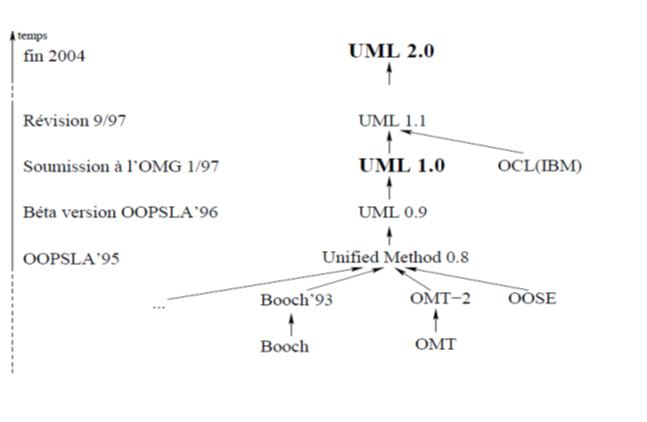
\includegraphics[width = 1\linewidth]{img/uml_historique.jpeg}
    \caption{Historique UML}
\end{figure}
UML 2 s’articule autour de treize types de diagrammes, chacun d’eux étant dédié à la
représentation des concepts particuliers d’un système logiciel. Ces types de diagrammes sont
répartis en deux grands groupes :

 \begin{itemize}
    \item \textbf{Six diagrammes structurels :}\\
    -- Diagramme de classes - Il montre les briques de base statiques : classes,
associations, interfaces, attributs, opérations, généralisations, etc.\\
    --  Diagramme d’objets - Il montre les instances des éléments structurels et
leurs liens à l’exécution.\\
    -- Diagramme de paquetages - Il montre l’organisation logique du modèle
et les relations entre packages.\\
   -- Diagramme de structure composite - Il montre l’organisation interne
d’un élément statique complexe.\\
    -- Diagramme de composants - Il montre des structures complexes, avec
leurs interfaces fournies et requises.\\
    -- Diagramme de déploiement - Il montre le déploiement physique des «
artefacts » sur les ressources matérielles.
    \item \textbf{Sept diagrammes comportementaux :}\\
    -- Diagramme de cas d’utilisation - Il montre les interactions fonctionnelles
entre les acteurs et le système à l’étude.\\
    -- Diagramme de vue d’ensemble des interactions - Il fusionne les
diagrammes d’activité et de séquence pour combiner des fragments
d’interaction avec des décisions et des flots.\\
    -- Diagramme de séquence - Il montre la séquence verticale des messages
passés entre objets au sein d’une interaction.\\
    -- Diagramme de communication - Il montre la communication entre objets
dans le plan au sein d’une interaction.\\
    -- Diagramme de temps - Il fusionne les diagrammes d’états et de séquence
pour montrer l’évolution de l’état d’un objet au cours du temps.\\
    -- Diagramme d’activité - Il montre l’enchaînement des actions et décisions
au sein d’une activité.\\
    -- Diagramme d’états - Il montre les différents états et transitions possibles
des objets d’une classe.
\end{itemize}

\subsubsection{Choix d'une méthode  d'analyse et de conception}
Afin de réaliser un bon système, une étude et une conception normalisée selon la norme de
modélisation universellement reconnue polyvalente et performante,\\ l’utilisation d’UML
s’avère nécessaire.\\
Dans notre démarche, pour la réalisation du système du projet, nous retenons les étapes
suivantes :

 \begin{itemize}
    \item détermination des acteurs potentiels du système
    \item description des cas d’utilisation fondamentaux
    \item les diagrammes de séquence
    \item le diagramme de classe de conception
\end{itemize}



%CHAPITRE 2
\chapter{ Etude de l'existant }
\textit{\textbf{Résumé:} }
\setcounter{minitocdepth}{1}
\minitoc

\section{Définitions des concepts du domaine}
Dans cette section nous allons définir certains concepts clés qui s'articule autour de notre sujet.
\subsection{Qu’est-ce que le e-commerce ?}
Dans l’absolu, l’e-commerce, c’est-à-dire le commerce électronique, désigne simplement l’achat et la vente de produits et services sur Internet. Cependant, le terme est souvent utilisé pour décrire toutes les mesures et actions entreprises par un vendeur dans le but de vendre des produits directement aux consommateurs. Le processus démarre dès qu’un client potentiel découvre un produit, l’achète et l’utilise jusqu’à, idéalement, devenir un client fidèle.
\begin{figure}[H]
    \centering
    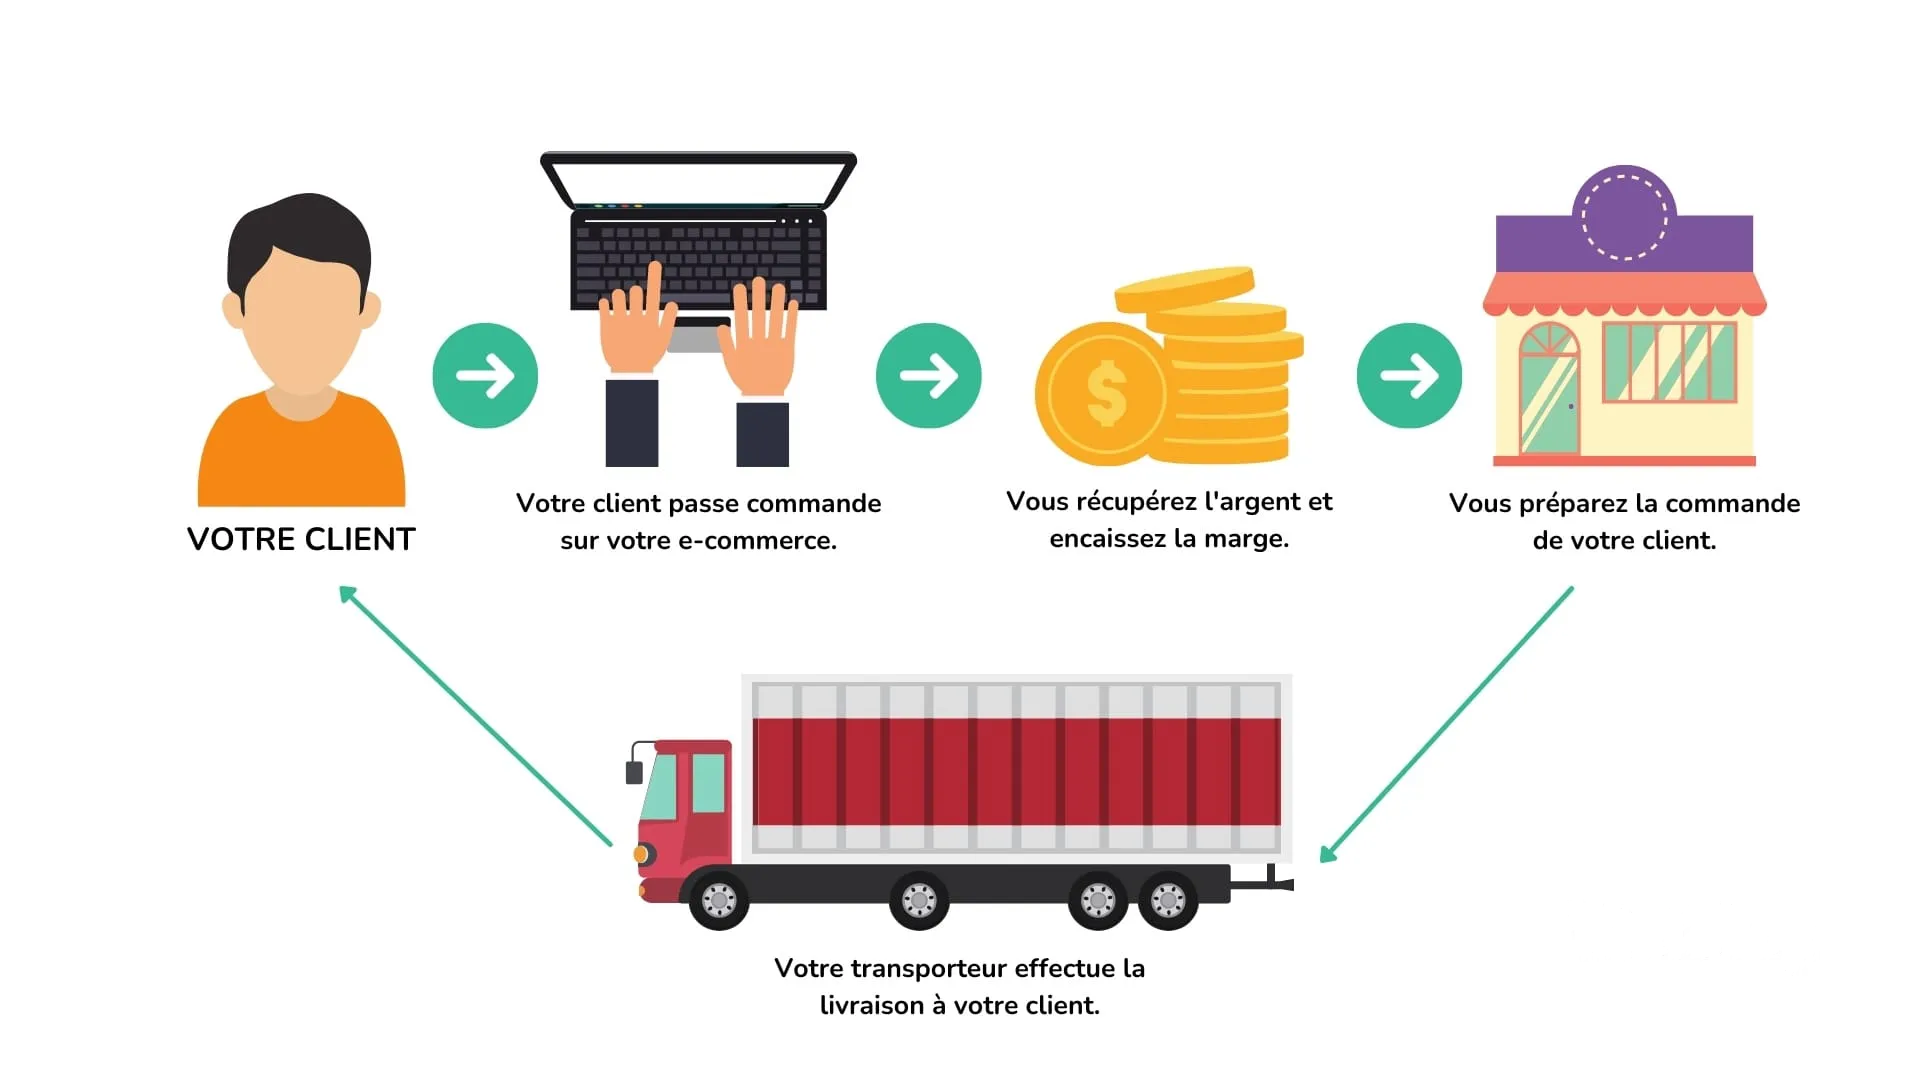
\includegraphics[width = 1\linewidth]{img/how-e-commerce.png}
    \caption{E-commerce}
\end{figure}
\subsubsection{5 outils d'e-commerce disponible sur le marché : } 
\textbf{-- WooCommerce :}\\
WooCommerce détient la plus grande part de marché de toutes les plateformes e-commerce. Comme le service fonctionne sur WordPress, vous devez maîtriser la technologie et vous familiariser avec ce CMS. Si vous n'êtes pas familier à WordPress, la configuration d'une boutique en ligne WooCommerce peut ne pas vous convenir.Le service comprend une grande variété d'extensions afin que vous puissiez adapter votre boutique en ligne à vos besoins commerciaux les plus spécifiques. Cependant, cette plateforme e-commerce manque d'évolutivité. À mesure que le nombre de clients et de commandes augmente, le temps de réponse de votre site Web ralentira.\\

Pour vous aider à mesurer les performances de votre entreprise, WooCommerce consolide les données sur vos revenus, clients, produits, taxes, etc. Dans l'exemple ci-dessous, vous pouvez voir les résultats des revenus pour une période choisie et les comparer avec les résultats de l'année précédente sur le graphique.
\begin{figure}[H]
    \centering
    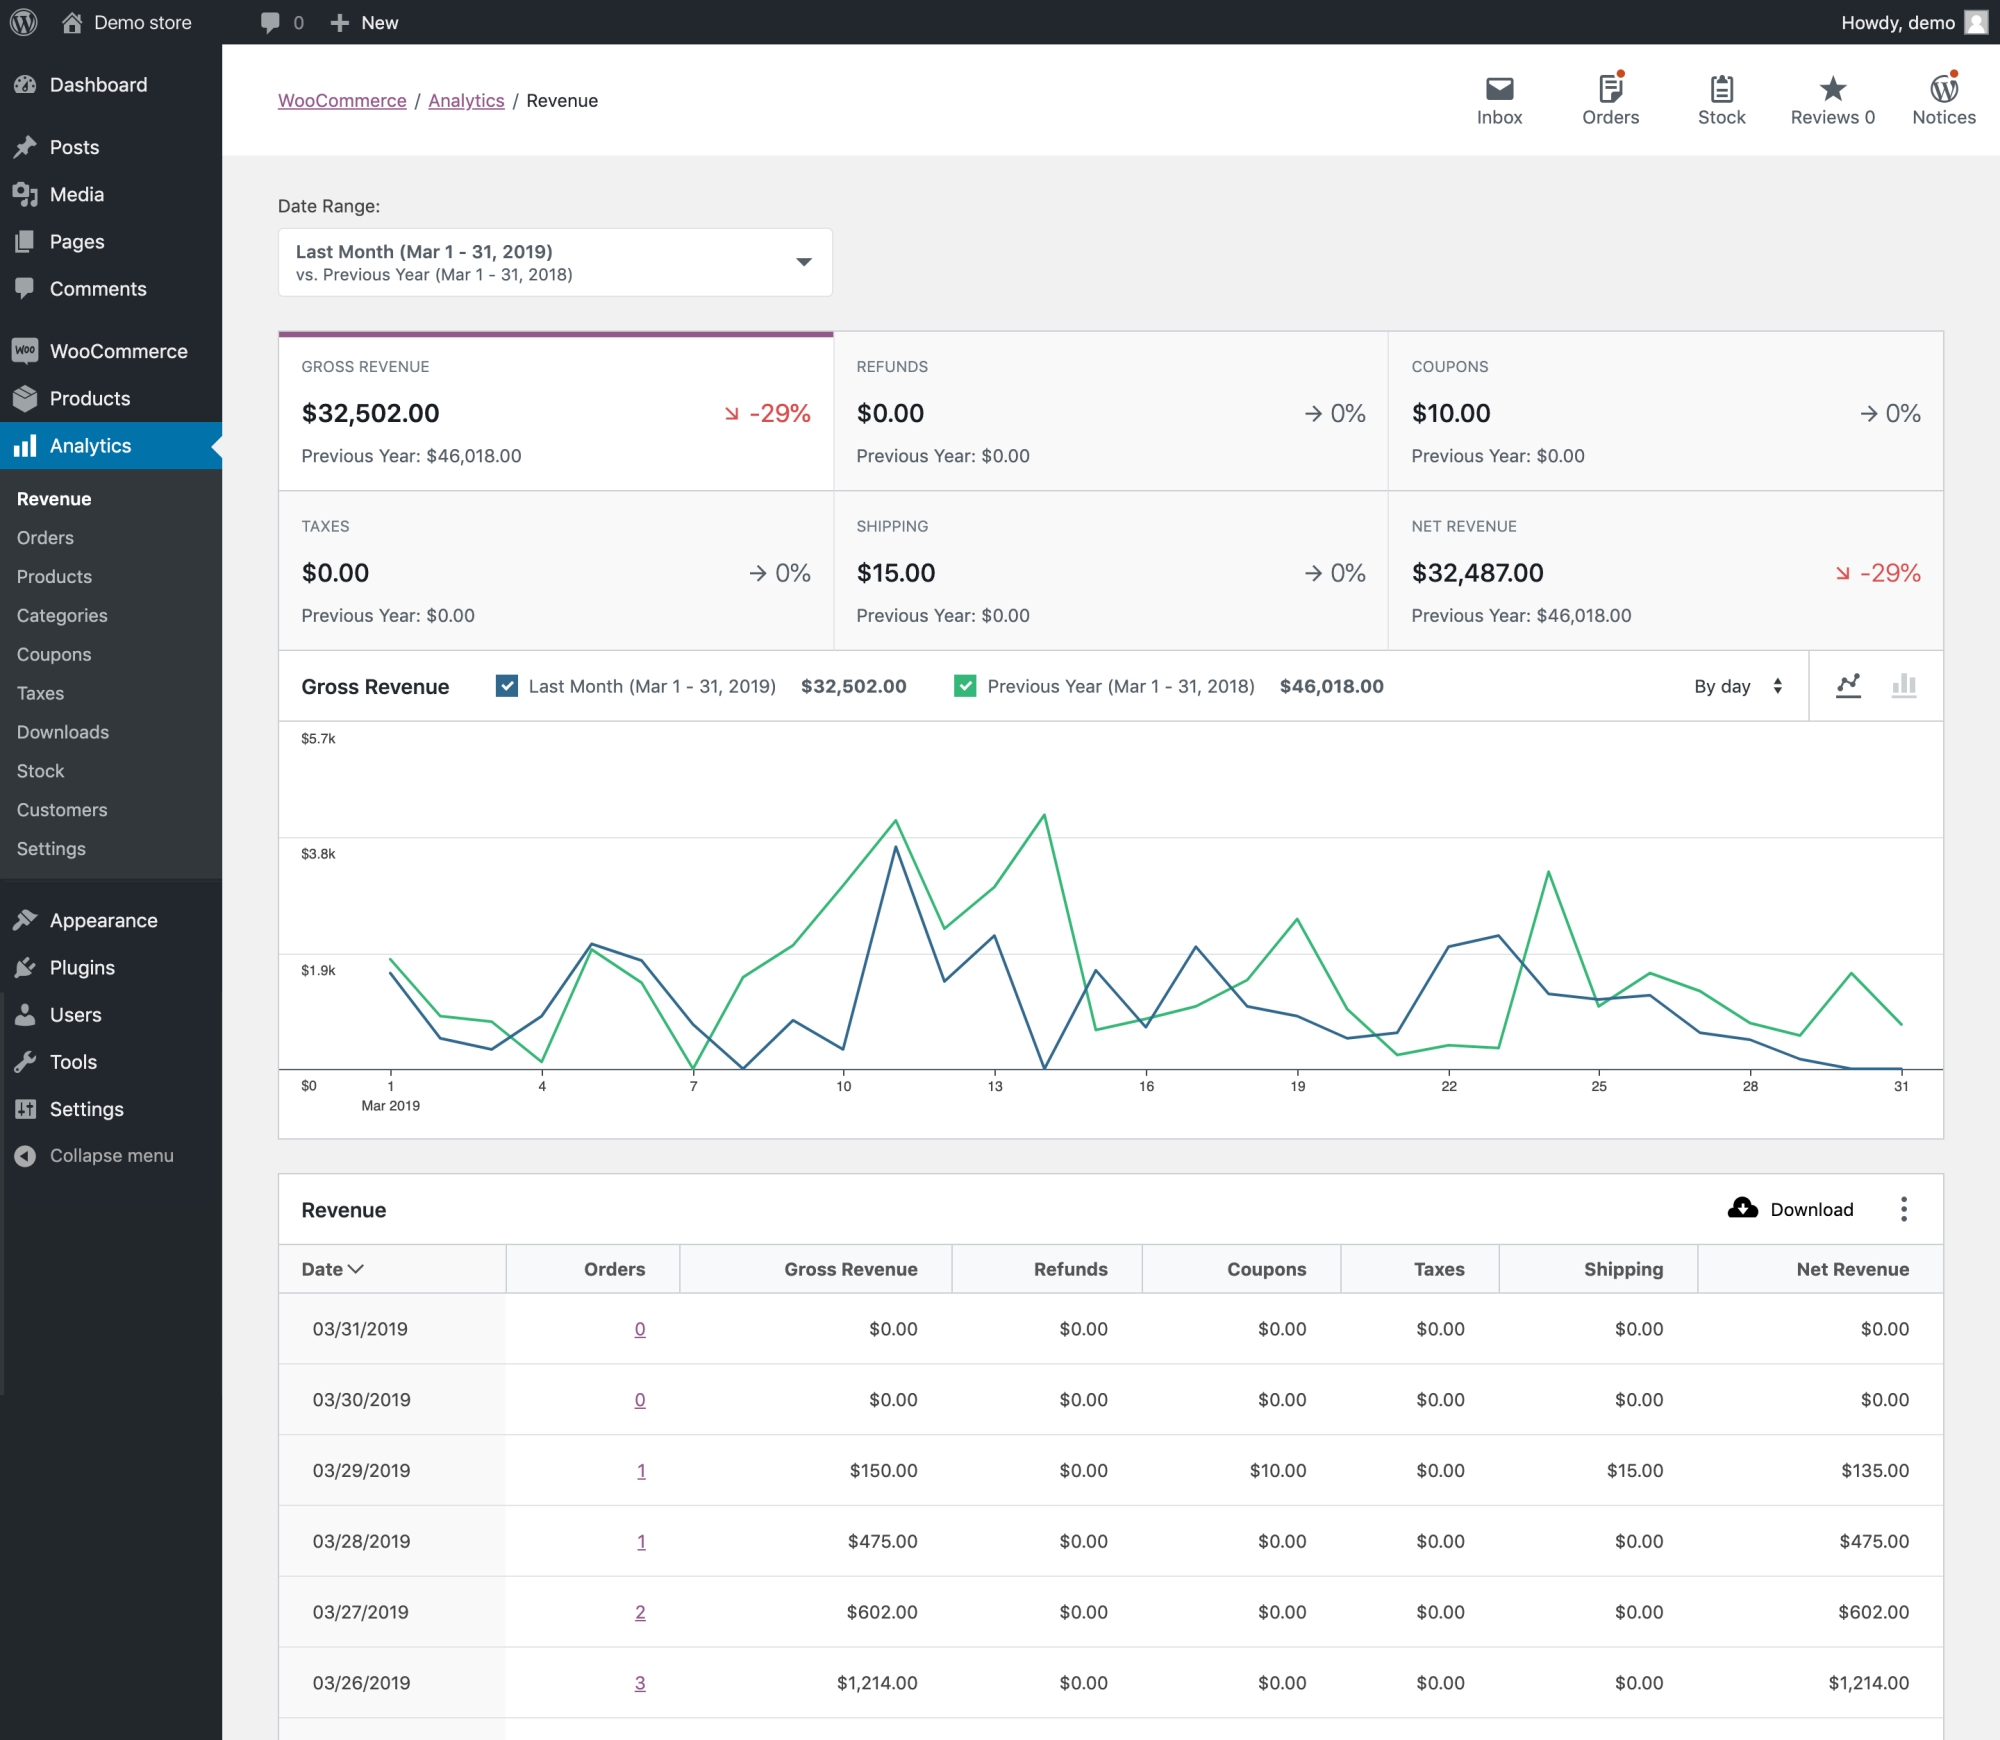
\includegraphics[width = 1\linewidth]{img/ecommerce-platform-woocommerce.png}
    \caption{Tableau de bord WooCommerce.}
\end{figure}

\textbf{-- Boutiques Wix :}\\
Wix est un créateur de sites Web et de pages de destination bien connu qui a ajouté des fonctionnalités de commerce électronique au cours des dernières années. Le principal avantage de cette plateforme est son éditeur glisser-déposer et l'abondance de modèles de conception personnalisables. Le service propose même de créer automatiquement votre boutique en ligne via l'outil Wix ADI.\\
Cette plateforme e-commerce prend également en charge le référencement de votre boutique en ligne, en proposant un plan personnalisé. Parmi les autres fonctionnalités utiles, citons l'analyse approfondie des performances du site, les outils de marketing SMM et email et une multitude d'options d'intégration.\\
L'un des inconvénients de ce service est son stockage relativement faible, ce qui fait de Wix une solution inadaptée aux grandes entreprises ou à croissance rapide. Cependant, le service fournit une assistance en ligne pendant la configuration, ainsi qu'une assistance téléphonique et par chat 24h/24 et 7j/7.

L'interface de Wix Stores est simple. Le tableau de bord principal vous montre le revenu total, le nombre de produits vendus et le montant des transactions.
\begin{figure}[H]
    \centering
    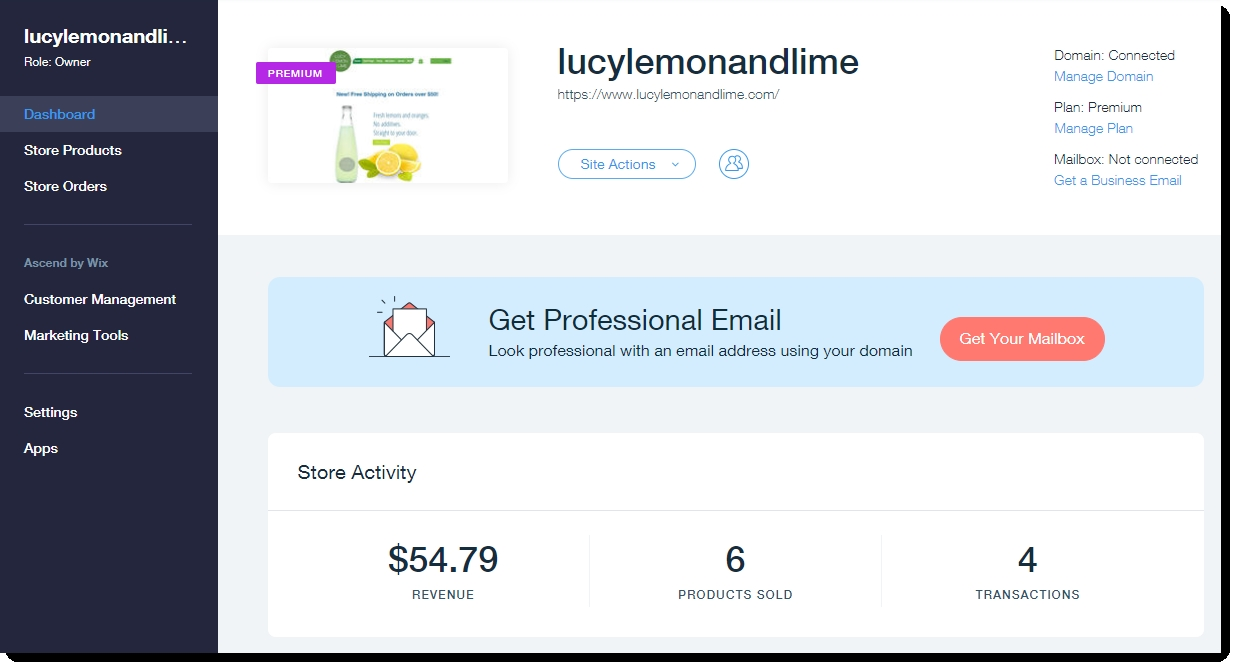
\includegraphics[width = 1\linewidth]{img/ecommerce-platform-wix_stores.png}
    \caption{Tableau de bord Wix Stores.}
\end{figure}

\textbf{-- Shopify}\\
L'une des plateformes e-commerce les plus connues, Shopify, propose un éditeur intuitif par glisser-déposer pour la création de sites Web. Les options de design incluent 9 thèmes prédéfinis gratuits et 64 payants triés par secteur d'activité, style visuel, etc.\\
Parmi les autres avantages de cette plateforme e-commerce, citons un système de gestion des expéditions, des prix spéciaux pour les services de transporteur, des analyses avancées, etc. Pour vous aider à gérer tous ces outils, Shopify propose une équipe d'assistance, un centre d'aide et une poignée de forums.\\
Shopify vous donne toutes les informations essentielles sur votre entreprise en temps réel. Dans l'image ci-dessous, l'onglet Accueil affiche les ventes, les commandes, les sessions et le nombre de visiteurs d'aujourd'hui. Connaissant les canaux les plus performants et les meilleurs produits, vous pouvez ajuster vos tactiques pour améliorer les performances


\begin{figure}[H]
    \centering
    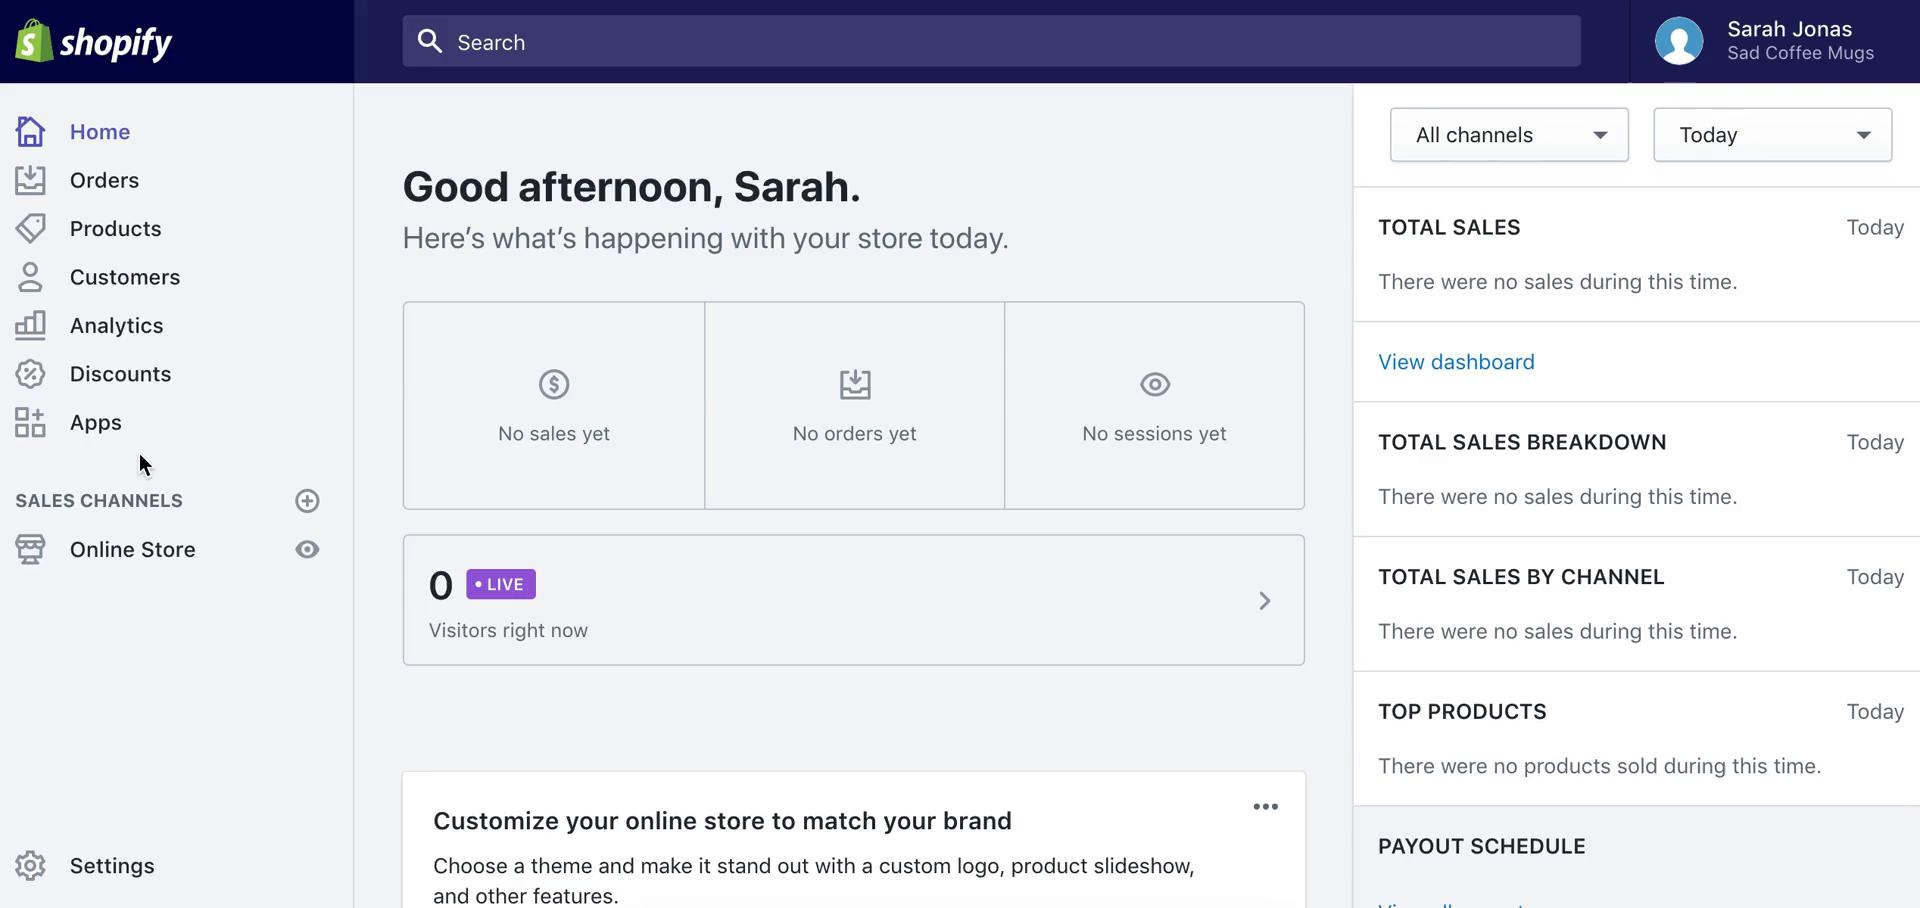
\includegraphics[width = 1\linewidth]{img/o.png}
    \caption{Onglet Accueil Shopify.}
\end{figure}

\textbf{-- BigCommerce}\\
Cette plateforme e-commerce est une excellente solution pour les grandes marques et les magasins physiques qui souhaitent accepter des commandes en ligne. Le service offre une grande variété de solutions marketing prêtes à l'emploi. Ils incluent un référencement de haute qualité, la possibilité de lancer un blog, un économiseur de panier abandonné, des fonctionnalités de marketing par e-mail, etc.\\

Vous pouvez commencer à créer votre site Web en choisissant l'un des nombreux thèmes préconçus. Accédez-y via l'interface BigCommerce, triez par secteur d'activité ou par prix, comme indiqué sur l'image. Pour ajuster les modèles, vous n'avez besoin d'aucune compétence technique. Cependant, il existe des possibilités de personnalisation avancées disponibles avec l'éditeur HTML et CSS.


\begin{figure}[H]
    \centering
    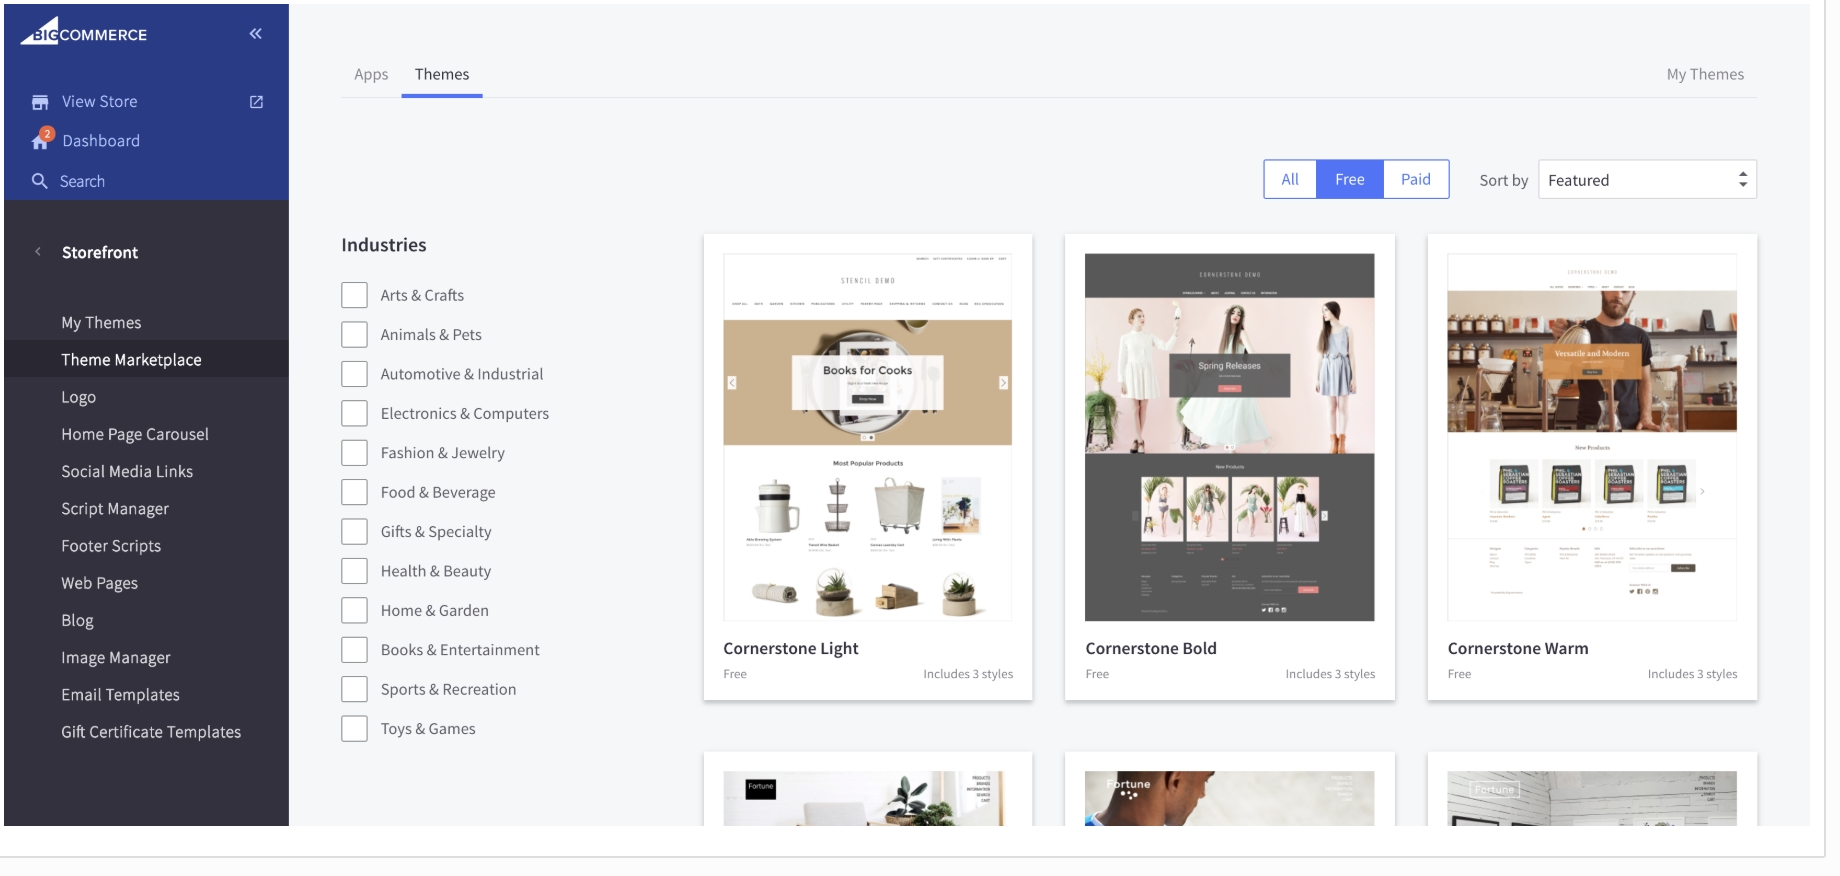
\includegraphics[width = 1\linewidth]{img/bigcom.png}
    \caption{Interface BigCommerce.}
\end{figure}

\textbf{-- PrestaShop}\\
PrestaShop est une autre plateforme e-commerce qui nécessite des compétences techniques. Pour configurer une boutique en ligne avec ce service, vous avez besoin de connaissances en HTML, CSS ou PHP. Une autre option à envisager est de recruter un développeur. PrestaShop vous fournit des agences partenaires à contacter.\\

Ce service de commerce électronique vous fournit des analyses approfondies, comme vous pouvez le voir ci-dessous. Le tableau de bord comprend des données sur les ventes, les commandes, la valeur du panier, les visites, le taux de conversion, les bénéfices, etc.

\begin{figure}[H]
    \centering
    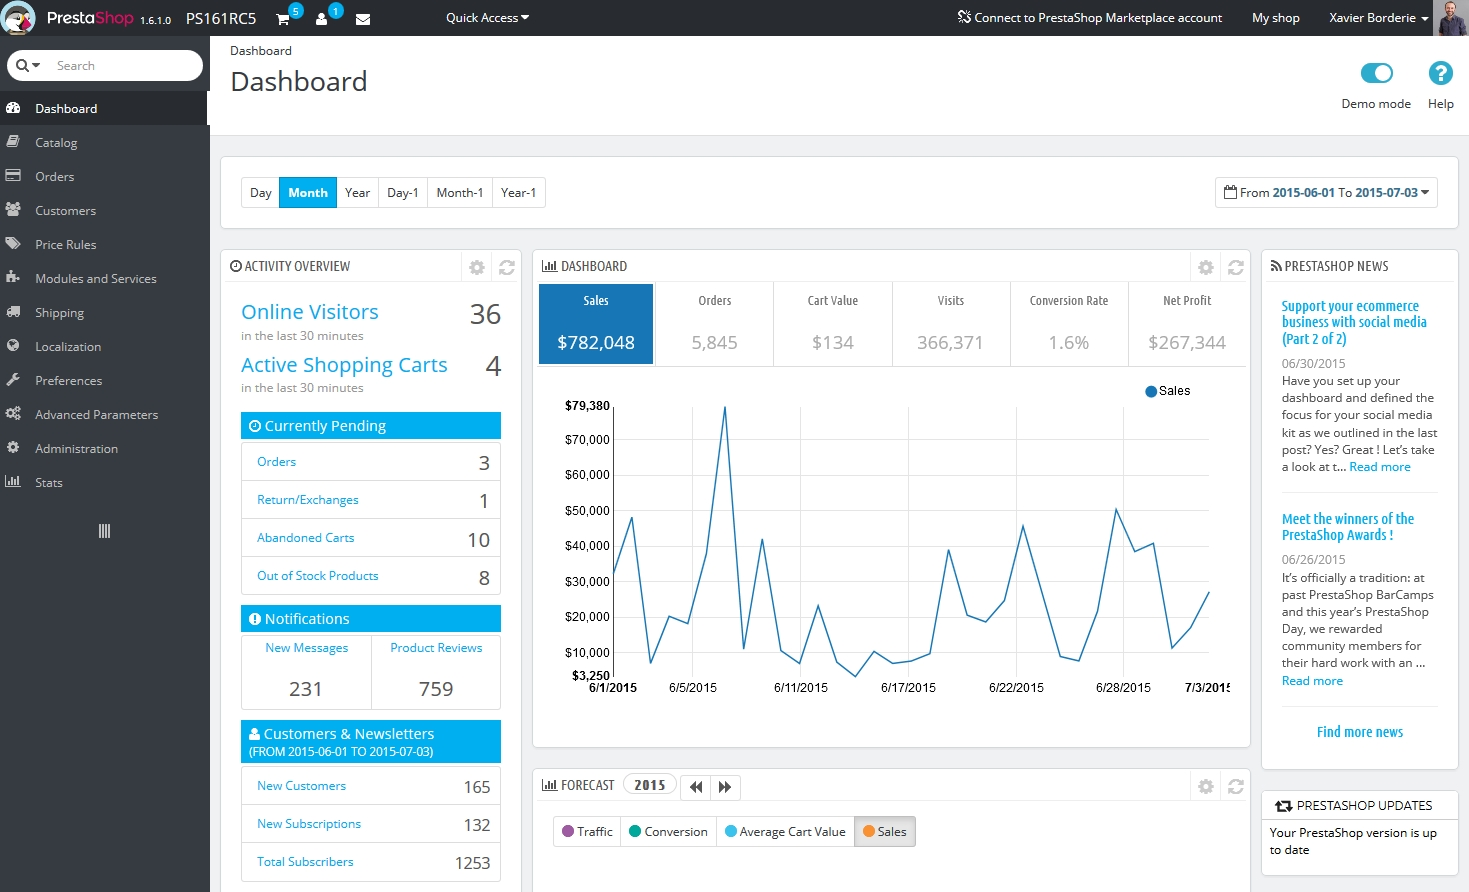
\includegraphics[width = 1\linewidth]{img/ecommerce-platform-prestashop.png}
    \caption{Tableau de bord PrestaShop.}
\end{figure}

\subsection{Qu’est-ce que la Business Intelligence ou BI (informatique décisionnelle) : }
Le terme Business Intelligence (BI) désigne les technologies, applications et pratiques de collecte, d'intégration, d'analyse et de présentation de l'information. L'objectif de la Business Intelligence est de soutenir une meilleure prise de décision des verticales métiers, commerciale, marketing, finance. Essentiellement, les systèmes de Business Intelligence sont des systèmes d'aide à la décision axés sur les données.La Business Intelligence englobe une grande variété d'outils, d'applications et de méthodologies qui permettent aux organisations de collecter des données à partir de systèmes internes et de sources externes. Ces données sont ensuite préparées pour l'analyse afin de créer des rapports, tableaux de bord et et autres outils de de Data Viz pour rendre les résultats analytiques disponibles aux décideurs et aux opérations.Aujourd'hui, les entreprises s'appuient sur les logiciels de Business Intelligence pour identifier et extraire des informations précieuses des grands volumes de données qu'elles stockent. Ces outils permettent d’en tirer des informations tels que des veilles concurrentielles et les tendances du marché, ainsi que des informations internes tel que trouver les raisons des opportunités perdues.
\begin{figure}[H]
    \centering
    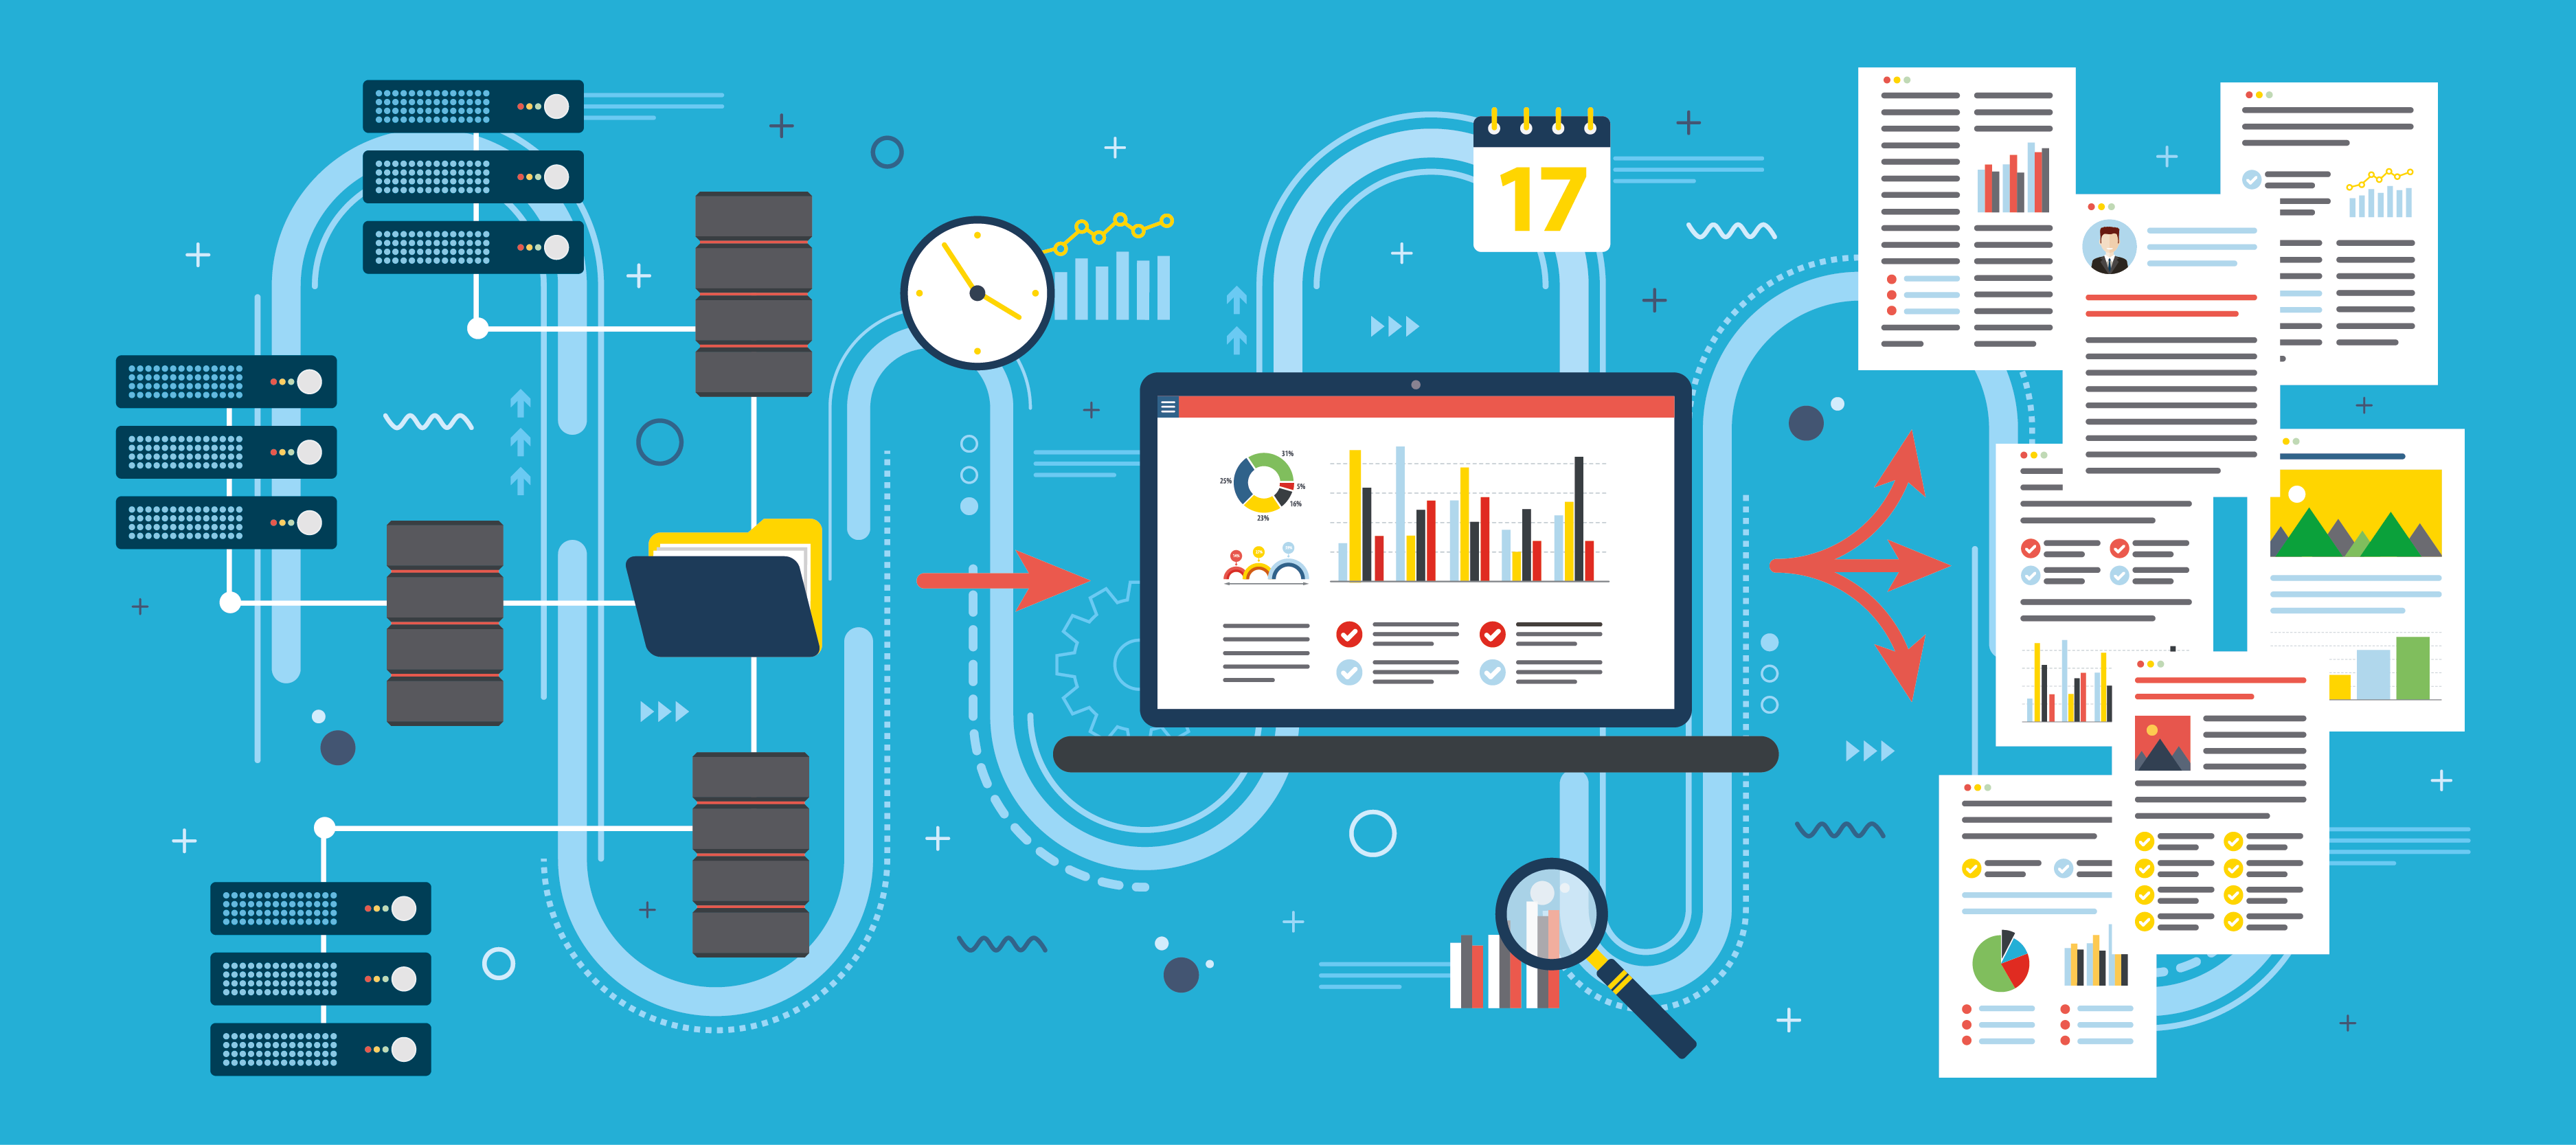
\includegraphics[width = 1\linewidth]{img/business-intelligence-4-01.png}
    \caption{Business Intelligence.}
\end{figure}
\section{Fonctionnalités existantes}

\subsection{Les acteurs principaux}
\subsection{Les modules existants}


%CHAPITRE 3
\chapter{Spécifications fonctionnelles détaillées}
\textit{\textbf{Résumé:}}
\setcounter{minitocdepth}{2}
\minitoc
\section{Les acteurs de l'application}
\section{Présentation du domaine}


%CHAPITRE 4
\chapter{Conception de la plateforme}
\textit{\textbf{Résumé : }}
\setcounter{minitocdepth}{1}
\minitoc
\newpage
\section{Architecture logique}

\section{Choix technologiques}

\section{Architecture technique}


\textit{\textbf{Résumé:} }
\minitoc
\newpage

%CHAPITRE 5
\chapter{Implémentation de la solution}

\textit{\textbf{Résumé:} }
\minitoc
\newpage
\section{Architecture de la solution}
\section{Présentation de l'application}



\chapter*{Conclusion et Perspectives} \mtcaddchapter
\markboth{Conclusion et Perspectives}{}
\addcontentsline{toc}{chapter}{Conclusion et Perspectives}

\bibliographystyle{plain}
\bibliography{biblio}

\chapter*{Annexes} \mtcaddchapter
\addcontentsline{toc}{chapter}{Annexes}
\markboth{Annexes}{}
\newpage


\section*{Résumé \markboth{}{}}
\thispagestyle{empty}


\section*{Abstract \markboth{}{}} 

\end{document}
